%Teori 1/5
%I teorikapitlet skal du plassere din studie inn i et overordnet teoretisk rammeverk. Formålet med dette kapitlet er å gjøre rede for de spesifikke teoriene og begrepene du anvender senere i avhandlingen. Du bør også begrunne hvorfor de er viktige for din studie. Du skal vise at du har forstått teorien du skal anvende. Pass på å bare skrive om det du bruker i analysen eller i tolkningen av datamaterialet.

%Det er verdt å merke seg at ikke alle oppgaver har en egen teoridel. Benytter du deg av IMRoD-modellen, har du presentert tidligere forskning i introduksjonen.

%Dette stoffet skal ha tilknytning til arbeidet som er gjort og gi det bakgrunnsstoffet som er nødvendig for å vurdere resultatene. Kapitlet kan for eksempel omfatte beskrivelse av råvarer/ ingredienser, fremstillingsmetoder, analysemetoder, tidligere arbeider innen temaet, kjemiske ligninger, økonomiske beregninger og sensoriske metoder. Det er ikke nødvendig å ha med mye generelt stoff – lærebokstoff – det kan gi inntrykk av at man ikke behersker emnet man har arbeidet med. 

%NVIDIA’s platforms and application frameworks enable developers to build a wide array of AI applications. Consider potential algorithmic bias when choosing or creating the models being deployed. Work with the model’s developer to ensure that it meets the requirements for the relevant industry and use case; that the necessary instruction and documentation are provided to understand error rates, confidence intervals, and results; and that the model is being used under the conditions and in the manner intended.

\section{Teori} 

%bakgrunnen for valg av tema
%problemstillingen eller hypotesene du skal undersøke
%På slutten av introduksjonen kan du også si noe om hvordan du har tenkt å strukturere resten av oppgaven, som en kort leserguide.

%Et tips er å begynne å skrive på innledningen tidlig, slik at den kan gi retning for det videre arbeidet ditt. Så går du heller over innledningen igjen på slutten for å skrive den helt ferdig. Da får du en innledning som har god sammenheng med resten av teksten.

\subsection{Bakgrunn}
\label{part:background}
%\begin{figure}
%\begin{center} 
%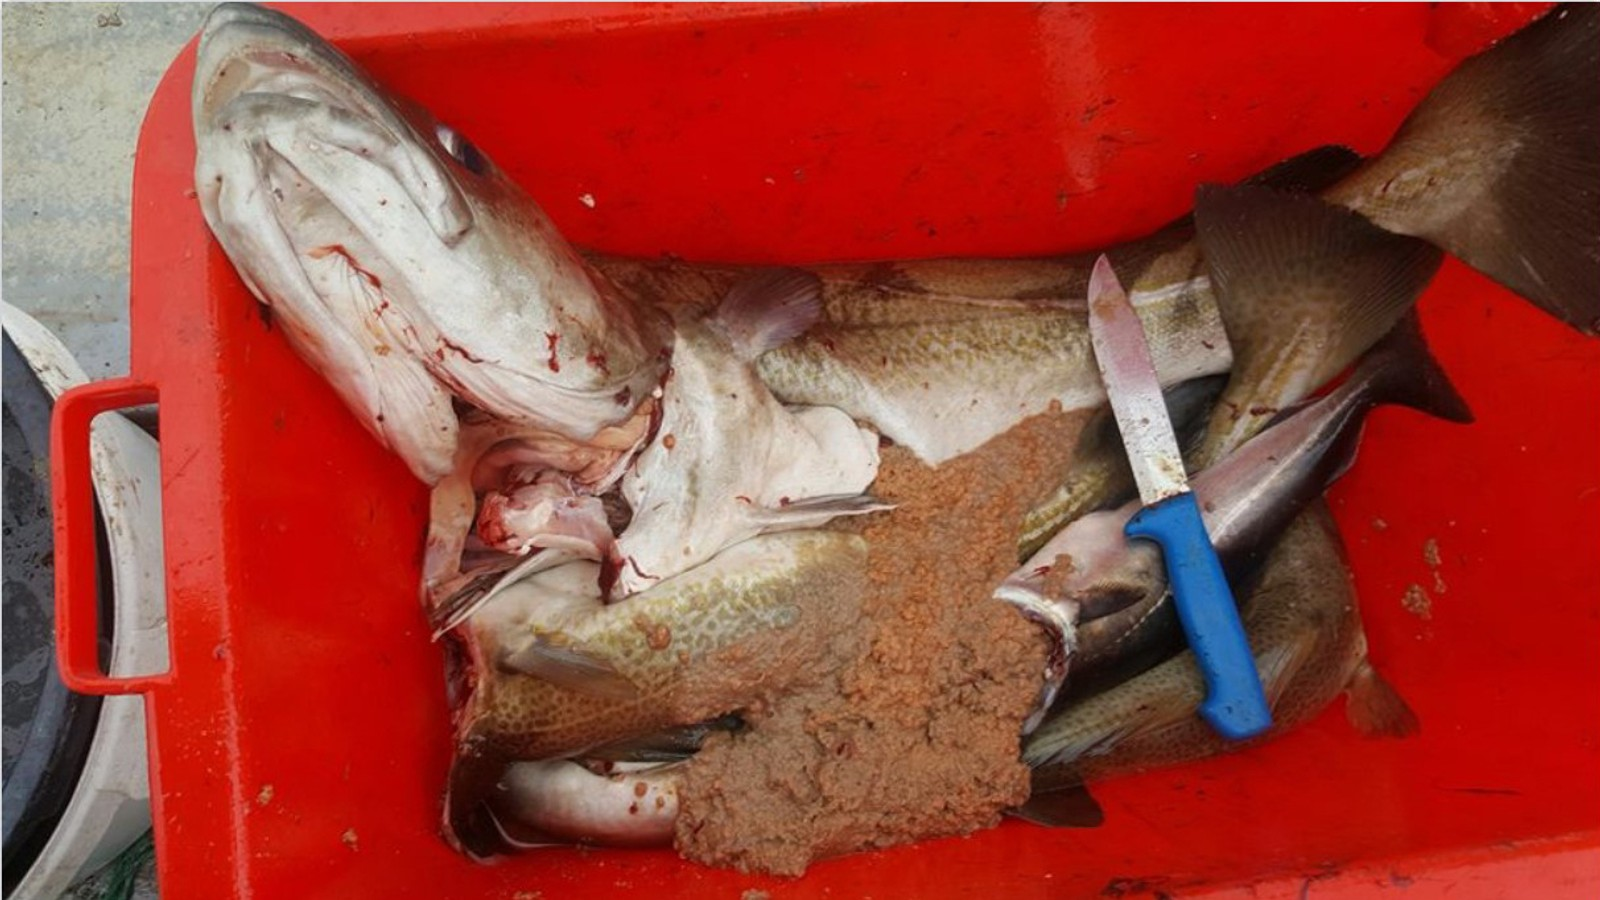
\includegraphics[scale=0.2]{figures/forsprengt}
%\caption{\small \sl Figuren viser et eksempel av fôrsprengt fisk. Det lukter ekkelt og det er forferdelig å sløye en fôrsprengt fisk, ifølge flere fiskere som har vært i kontakt med NRK. Foto: Arnold Jensen. \cite{Trana m.fl. 2019} \label{fig:forsprengt}} 
%\end{center} 
%\end{figure} 

Kystfiskere hevder villfisken får i seg så mye laksefôr at fiskeplassene blir ødelagt. Fisker Tor Inge Larsen i Brønnøysund sa til NRK i 2018 at han fortviler over det han mener er dårligere kvalitet hos fisken han fanger. Han sa han kan knapt huske sist han fikk en sei om bord i båten uten at den hadde pellets fra lakseoppdrett i magen. Han hevder fiskerne har blitt frastjålet fiskeområder på høylys dag, og mener fiskefeltene nært Brønnøysund på Sør-Helgeland i Nordland har fått betydelig lavere kvalitet på grunn av oppdrettsanleggene. \cite{Olsen m.fl. 2018}

Kommunikasjonsdirektør Are Kvistad i Sjømat Norge er litt overrasket over utspillet fra fiskeren på Helgeland. Han mener laksepellets ikke utgjør noen fare for villfisk. «Det er et fiskefôr som blir sjekket av myndighetene, og er et trygt og næringsrikt fôr som også er trygt for villfisk», sa Kvistad til NRK i 2018. Kvistad mente det også er i oppdretternes interesse, både økonomisk og utslippsmessig, å redusere fôringen av oppdrettslaksen slik at den kun får den maten den trenger. \cite{Olsen m.fl. 2018}

%Hvis jeg kan foreslå en mulig forbedring så kan første del av avsnitt 1.1 skrives litt mer sammenfattet, for eksempel med et par avsnitt om hvilke grupper som er negative til «pelletsfisk», og et par avsnitt om hvem som er positive eller likegyldig til det. Her kan du også vise til en spørreundersøkelse som er gjort på sameksistensprosjektet. Den er ikke publisert enda, men forskerne har skrevet en bloggartikkel om den https://blogg.forskning.no/fra-fjord-til-bord/hvem-bryr-seg-om-pelletssei/1648846.

Men ikke alle er negative til «pelletsfisk». Nofima gjorde en undersøkelse i 2020 som viser hvilke grupper som er negative, positive eller likegyldig til fisken. Nofima-forskerne Anette Hustad og Ragnhild Svalheim oppdaget at de fleste er nøytrale til påstander om at pelletssei smaker eller lukter annerledes enn annen sei. \cite{Hustad og Svalheim 2020}

\begin{figure} 
\begin{center} 
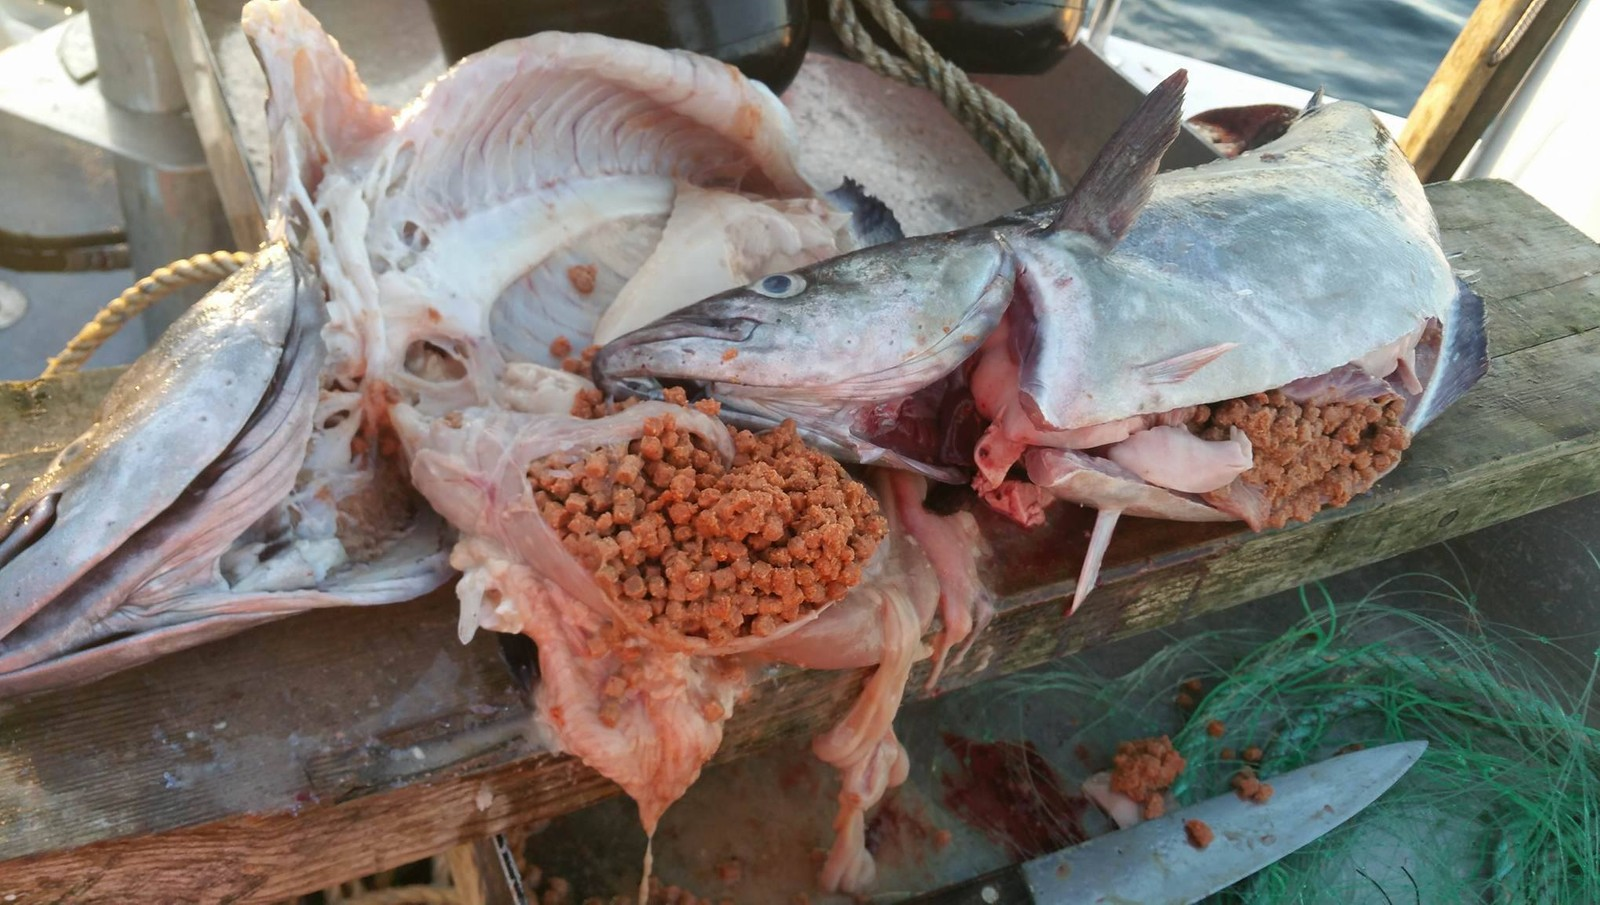
\includegraphics[scale=0.2]{figures/oppdrettfor}
\caption{\small \sl Figuren viser et eksempel av «pellets-fisken». Det lukter ekkelt og det er forferdelig å sløye en fôrsprengt fisk, ifølge flere fiskere som har vært i kontakt med NRK \cite{Trana m.fl. 2019}. Seien har vært under merdene, da blir den full av pellets. Fôrsprengt fisk er unaturlig, hode blir for liten og kroppen for stor. Dette har pågått i mange år. Likevel blir fisken omsatt, fiskere får levert slik fisk til enkelte fiskebruk. \cite{Angell og Ekanger 2017} \label{fig:oppdrettfor}} 
\end{center} 
\end{figure} 

Det er forsket relativt lite på hvordan oppdrett påvirker villfisk, men seniorrådgiver Bjørn-Steinar Sæther fra Nofima ga ut en artikkel i 2017 der han viste at seien som hadde spist oppdrettsfôr får en litt bløtere og noe mer spaltet muskel enn annen sei. Ellers var kvaliteten fortsatt stort sett innenfor kategorien god kvalitet. \cite{Saether 2017}

%Det kan også være greit å legge mer vekt på at oppdrettsnæringen er interessert i å kartlegge hvor mye fôr som spises av villfisk. Det er viktig for dem å ha kontroll på fôrmengden som går til spille siden det er en stor kostnad som har økt mye de siste årene (se f. eks. https://www.fhf.no/nyheter/nyhetsarkiv/kostnadene-for-norsk-lakseoppdrett-fortsetter-aa-oeke-ogsaa-i-2019/). Man kan derfor si at dette prosjektet vil være positivt for både fiskere og oppdrettere.

Oppdrettsnæringen er også interessert i å kartlegge hvor mye fôr som spises av villfisk. I 2019 avsluttet FHF, Fiskeri- og havbruksnæringens forskningsfinansiering, et prosjekt ledet av Audun Iversen fra Nofima der de så på kostnadsutvikling og forståelse av drivkrefter i norsk lakseoppdrett. For oppdrettsnæringen er å ha kontroll på fôrmengde som går til spille viktig, fôrpellets er en stor kostnad som har økt mye de siste årene. De ønsker ikke å fôre oppdrettsfisken mer enn nødvendig. Om problemet løses så vil det bli mindre oppdrettsfôr til villfisken. \cite{Baevre-Jensen 2019}

%Johnny Eliassen som er bosatt på Reinøya i Troms, Karlsøy kommune, fortalte til NRK at han hadde tidligere engasjert seg i saken for å hindre at kystområdet ble lokasjon for oppdrettsanlegg. Det ble allikevel åpnet et oppdrettsanlegg mai 2017 i fjorden på Reinøya, og det hevder de lokale fiskerne at de har merket. De har fisket «pelletstorsk»,  torsk med magen full av pellets, selv over en kilometer unna anlegget. Oppdrettere reklamerer oppdrettsfisk som den absolutte beste fisken. Eliassen kunne ikke tenke seg er at det virkelig er tilfelle, for lukten og konsistensen på fisken gjør den uspiselig i hans øyne. \cite{Jakobsen 2017}

%Vinteren 2018 rømte 52 000 laks fra Marine Harvests oppdrettsanlegg i Nærøy kommune i Trøndelag. Ifølge Namdalsavisa inneholdt laksen medisiner mot innvollsorm. Mattilsynet gikk ut og sa at det var trygt å spise fisken, men at den ikke kunne omsettes videre. \cite{nrk 2018}

%Den rømte laksen hadde blitt gitt medisinfôr med praziquantel og skulle være i karantene i 14 dager. For fiskere, slik som Arnold Jensen, er denne informasjonen skremmende. Jensen er medlem av Naturvernforbundets fiske- og oppdrettsutvalg. Han ønsker at mattryggheten til villfisk som beiter ved oppdrettsanleggene skal kontrolleres. Se figur \ref{fig:oppdrettfor} og \ref{fig:forsprengt}. \cite{Christensen 2019}

I 2019 kom «pellets-fisken» i medienes søkelys igjen, denne gangen var det fiskere i Lyngen kommune i Troms som slo alarm. Villfisk som hadde spist oppdrettsfôr som inneholdt medisin ble omsatt av fiskere i fjorden. Oppdrettsfisken var i karantene i denne perioden. Fiskerne ønsket svar på om villfisken kan være farlig for forbrukere. \cite{Trana m.fl. 2019}

%\begin{figure} 
%\begin{center} 
%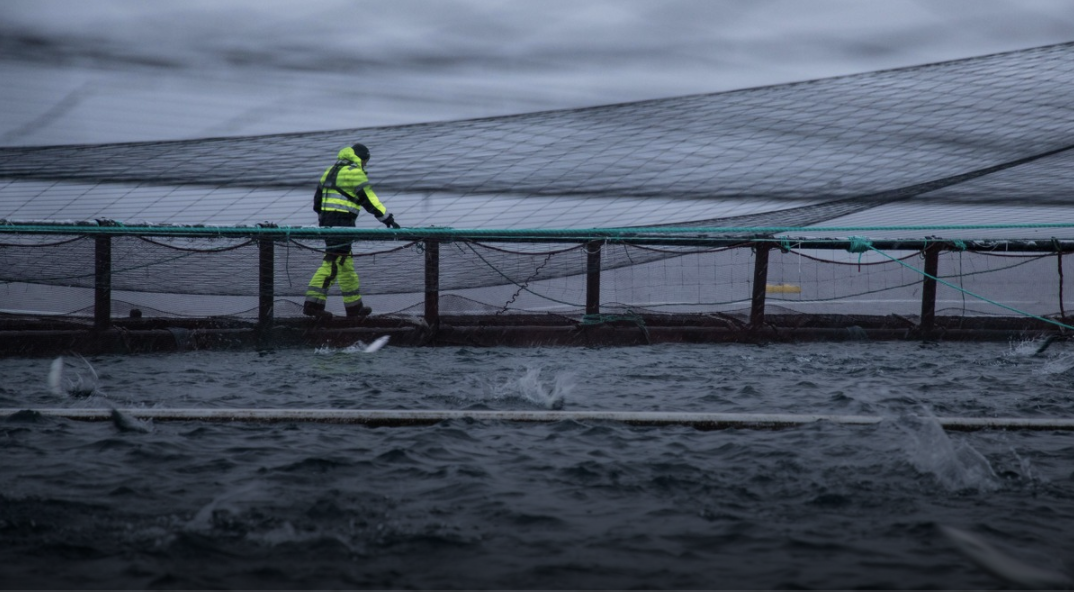
\includegraphics[scale=0.7]{figures/oppdrett}
%\caption{\small \sl Figuren viser et oppdrettsanlegg. Fôret oppdrettsfisken mates med spises også av villfisk. Oppdrettsbransjen er i konflikt med fiskere som mener oppdrettsnæringen ødelegger fiskeplasser i fjordene med anlegg og reduserer kvaliteten til villfisk som spiser fôrpellets under merdene. \cite{Olsen m.fl. 2018} \label{fig:anlegg}} 
%\end{center} 
%\end{figure} 

Sjømatdivisjonen og Akvadivisjonen ved Nofima har en strategisk internsatsing som går ut på å samle kunnskap om sameksistens mellom ulike marine næringer og interesser, deriblant om hvordan man kan unngå konflikter mellom ulike interesser. Se figur \ref{fig:anlegg}. \cite{Robertsen 2020}

En av problemstillingene er sameksistens mellom fiskeri- og oppdrettsnæringene, og hvordan oppdrettsanlegg påvirker de nærliggende fiskeplassene. I den forbindelse er det interessant å kartlegge omfanget av hvitfisk som beiter på fôr fra oppdrettsanlegg. Dette er en problemstilling som har vært i fokus hos media etter at flere fiskere har fanget fôrsprengt torsk og sei i fjorder hvor det finnes oppdrettsanlegg. Det hevdes at denne fisken er av betydelig dårligere kvalitet og den kan ha fått i seg medisiner gjennom fôret som gjør at den kan være farlig å spise. \cite{Olsen 2019}

Det behøves kunnskap om hvor mange villfisk som trekker til oppdrettsanlegg, og under hvilke forhold, slik at man kan komme nærmere en løsning som kan dempe konflikten mellom disse to næringene. 

Målet med dette prosjektet var å utvikle et system som kan telle antall villfisk av ulike arter basert på en videostrøm fra et undervannskamera. Det er ønskelig å kunne vise resultatet som en fordeling av observasjoner over tid for hver art.

\subsection{Kunstig intelligens}
\label{part:ai}

Kunstig intelligens (KI) er blitt et stort forskningsfelt med mange praktiske anvendelser og aktive forskningsprosjekter. Intelligent programvare automatiserer trivielt og repetitivt arbeid, forstår tale og kjenner igjen objekter i bilder, kan diagnosere pasienter innenfor medisin og hjelper forskere med grunnforskning. KI kan også finne mønstre i store datamengder som det er vanskelig for mennesker å få øye på. \cite{Goodfellow m.fl. 2016 s. 1}

\begin{figure} 
\begin{center} 
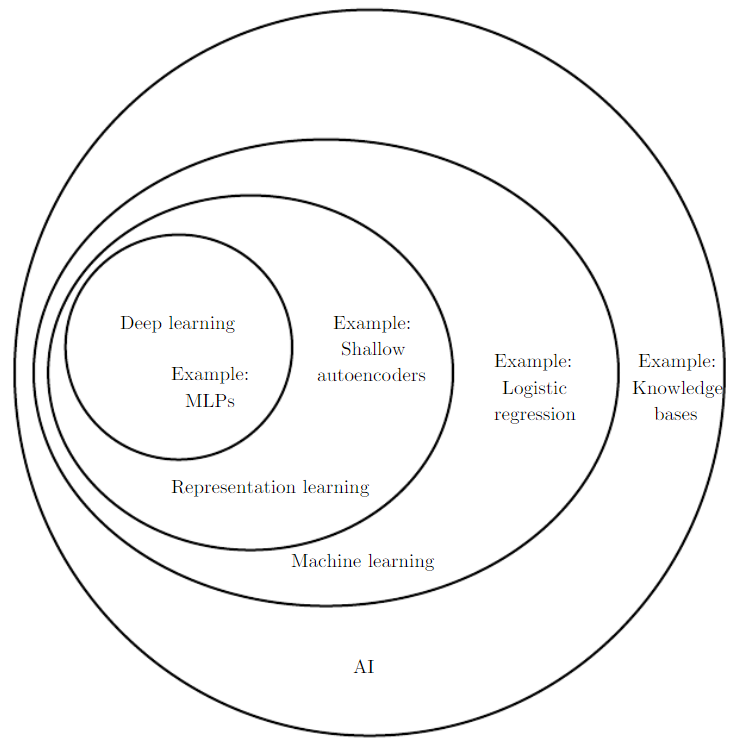
\includegraphics[scale=0.7]{figures/ai}
\caption{\small \sl Figuren viser et Venn diagram som viser at deep learning er en form for representativ læring, og det er igjen en form for maskinlæring. Maskinlæring er anvendt i mange, men ikke alle, de forskjellige metodene innenfor kunstig intelligens. Hver del av Venn diagrammet gir et eksempel av anvendelsen til teknologien. \cite{Goodfellow m.fl. 2016 s. 9} \label{fig:ai}} 
\end{center} 
\end{figure} 

\begin{figure} 
\begin{center} 
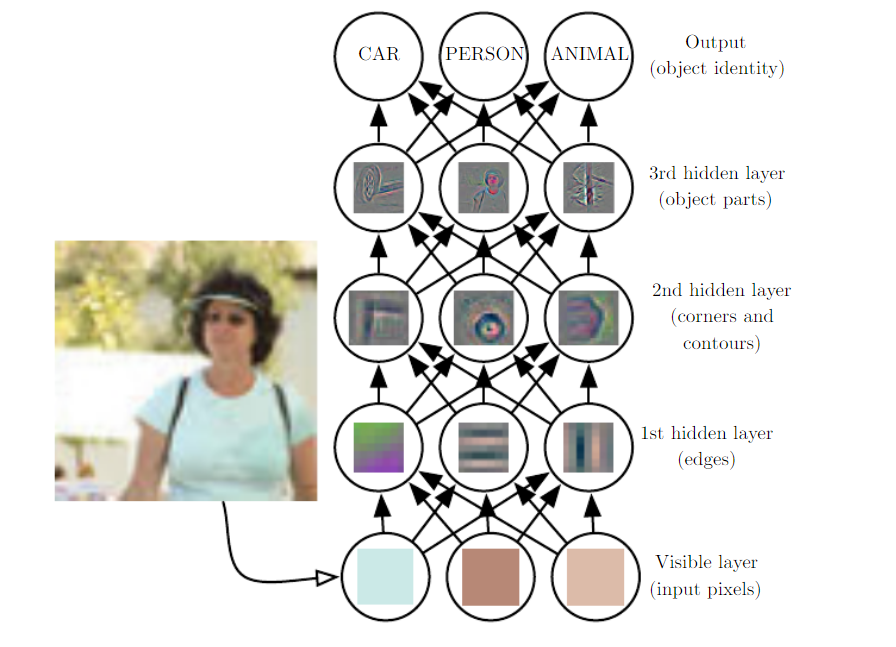
\includegraphics[scale=0.65]{figures/deep}
\caption{\small \sl Figuren viser en deep learning modell. Det er vanskelig for en datamaskin å forstå sensorisk rådata er. Å lage en funksjon som tar inn piksler og gir ut en objektidentitet er svært komplisert. Å utlede en slik funksjon virker nærmest umulig om en takler problemet direkte. Deep learning løser vanskelighetene ved dele opp den kompliserte funksjonenen til en samling sammenkoblede funksjoner. Disse funksjonene kalles ofte for kunstige nevroner, kerneler, perceptrons eller filtere. Utmatningene fra kernelene i ett lag blir innmatningene til neste lag i modellen. Innmatningen til modellen, slik som et bilde, kalles for det synlige laget, ettersom den består av informasjon som vi mennesker kan forstå. Dette laget er etterfulgt av en serie med skjulte lag, «hidden layers», hvert lag henter ut mer og mer abstrakte konsepter, «features», fra bildet. Disse lagene kalles for «hidden» ettersom verdiene i disse lagene ikke finnes i innmatningen til nettverket; modellen må selv bestemme hvilke konsepter som er nyttige for å beskrive sammenhengen i det synlige laget. Hvert lag danner forskjellig innsikt. Det første laget kan for eksempel lett gjenkjenne kantene i et bilde ved å sammenligne kontraster i bildet. Denne informasjonen sendes til det neste laget, et lag som finner kanter. Gitt det andre skjulte lagets beskrivelse av bildet, et bilde beskrevet med kanter, så kan objektdeteksjon bli mulig ved å sammenligne en samling kanter, konturer, med deler av kjente objekter. \cite{Goodfellow m.fl. 2016 s. 6} \label{fig:deep}} 
\end{center} 
\end{figure} 

Dette prosjektet beskriver maskiner som kan gi en tidsoversikt over torsk og sei fra en videostrøm. Den lærer konseptene en torsk eller sei består av, basert på data. Maskinlæring, å la en maskin lære fra data, er kun en av metodene innenfor kunstig intelligens. Se figur \ref{fig:ai}. \cite{Canziani m.fl. 2017 s. 1}

I begynnelsen løste kunstig intelligens problemer som var vanskelige for mennesker å løse, men relativt trivielle for datamaskiner. Utfordringen med kunstig intelligens viste seg å være å løse problemer som var enkle for mennesker å utføre, men vanskelige for mennesker å beskrive formelt. Problemer som vi løser intuitivt, som føles automatiske ut, slik som å forstå ordene til andre mennesker, ansiktene deres, og å kjenne igjen det en har sett tidligere i bilder. \cite{Goodfellow m.fl. 2016 s. 1}

Løsningen er å la datamaskiner lære fra erfaringer og forstå verden ved å forstå konsepter, som kan igjen bli forstått med enda enklere konsepter. Denne erfaringskunnskapen gjør datamaskinene selv, uten at et menneske formelt beskriver kunnskapen til maskinen. Erfaringene kan beskrives med en graf. Se figur \ref{fig:deep}. Ettersom denne grafen kan bestå av mange lag, den er dyp, så kalles denne formen for maskinlæring «deep learning» \cite{Goodfellow m.fl. 2016 s. 1}.

%"Deep Learning" is a general term that usually refers to the use of neural networks with multiple layers that synthesize the way the human brain learns and makes decisions. A convolutional neural network is a kind of neural network that extracts features from matrices of numeric values (often images) by convolving multiple filters over the matrix values to apply weights and identify patterns, such as edges, corners, and so on in an image. The numeric representations of these patterns are then passed to a fully-connected neural network layer to map the features to specific classes. https://notebooks.azure.com/graememalcolmoutlook/projects/mlprimers/html/05a%20-%20Image%20Classification%20with%20a%20CNN%20(PyTorch).ipynb

%The difficulties faced by systems relying on hard-coded knowledge suggestthat AI systems need the ability to acquire their own knowledge, by extracting2
%CHAPTER 1. INTRODUCTIONpatterns from raw data. This capability is known asmachine learning. Theintroduction of machine learning enabled computers to tackle problems involvingknowledge of the real world and make decisions that appear subjective. A simplemachine learning algorithm calledlogistic regressioncan determine whether torecommend cesarean delivery (Mor-Yosef et al., 1990). A simple machine learningalgorithm called naive Bayes can separate legitimate e-mail from spam e-mail \cite{Goodfellow m.fl. 2020 s. 3}

%The performance of these simple machine learning algorithms depends heavilyon therepresentationof the data they are given. For example, when logisticregression is used to recommend cesarean delivery, the AI system does not examinethe patient directly. Instead, the doctor tells the system several pieces of relevantinformation, such as the presence or absence of a uterine scar. Each piece ofinformation included in the representation of the patient is known as afeature.Logistic regression learns how each of these features of the patient correlates withvarious outcomes. However, it cannot influence how features are defined in anyway. If logistic regression were given an MRI scan of the patient, rather thanthe doctor’s formalized report, it would not be able to make useful predictions.Individual pixels in an MRI scan have negligible correlation with any complicationsthat might occur during delivery. \cite{Goodfellow m.fl. 2020 s. 3}

%This dependence on representations is a general phenomenon that appearsthroughout computer science and even daily life. In computer science, operationssuch as searching a collection of data can proceed exponentially faster if the collec-tion is structured and indexed intelligently. People can easily perform arithmeticon Arabic numerals but find arithmetic on Roman numerals much more timeconsuming. It is not surprising that the choice of representation has an enormouseffect on the performance of machine learning algorithms. For a simple visualexample, see figure 1.1.

%Many artificial intelligence tasks can be solved by designing the right set offeatures to extract for that task, then providing these features to a simple machinelearning algorithm. For example, a useful feature for speaker identification fromsound is an estimate of the size of the speaker’s vocal tract. This feature gives astrong clue as to whether the speaker is a man, woman, or child.

%For many tasks, however, it is difficult to know what features should beextracted. For example, suppose that we would like to write a program to detectcars in photographs. We know that cars have wheels, so we might like to use thepresence of a wheel as a feature. Unfortunately, it is difficult to describe exactlywhat a wheel looks like in terms of pixel values. A wheel has a simple geometricshape, but its image may be complicated by shadows falling on the wheel, the sunglaring off the metal parts of the wheel, the fender of the car or an object in the foreground obscuring part of the wheel, and so on.

%One solution to this problem is to use machine learning to discover not onlythe mapping from representation to output but also the representation itself.This approach is known asrepresentation learning. Learned representationsoften result in much better performance than can be obtained with hand-designedrepresentations. They also enable AI systems to rapidly adapt to new tasks, withminimal human intervention. A representation learning algorithm can discover agood set of features for a simple task in minutes, or for a complex task in hours tomonths. Manually designing features for a complex task requires a great deal ofhuman time and effort; it can take decades for an entire community of researchers.

%The quintessential example of a representation learning algorithm is theau-toencoder. An autoencoder is the combination of anencoderfunction, whichconverts the input data into a different representation, and adecoderfunction,which converts the new representation back into the original format. Autoencodersare trained to preserve as much information as possible when an input is runthrough the encoder and then the decoder, but they are also trained to make thenew representation have various nice properties. Different kinds of autoencodersaim to achieve different kinds of properties.

%A major source of difficulty in many real-world artificial intelligence applicationsis that many of the factors of variation influence every single piece of data we areable to observe. The individual pixels in an image of a red car might be very closeto black at night. The shape of the car’s silhouette depends on the viewing angle.Most applications require us to disentangle the factors of variation and discard theones that we do not care about.

%Deep learningsolves this central problem in representation learning by intro-ducing representations that are expressed in terms of other, simpler representations.Deep learning enables the computer to build complex concepts out of simpler con-cepts. Figure 1.2 shows how a deep learning system can represent the concept ofan image of a person by combining simpler concepts, such as corners and contours,which are in turn defined in terms of edges.

%The quintessential example of a deep learning model is the feedforward deepnetwork, ormultilayer perceptron(MLP). A multilayer perceptron is just amathematical function mapping some set of input values to output values. Thefunction is formed by composing many simpler functions. We can think of eachapplication of a different mathematical function as providing a new representationof the input.

%Programvaren implementeres i C++ ved hjelp av OpenCV-biblioteket. Det kan også være aktuelt å lage et grafisk grensesnitt hvor tellingene fra hver art kan vises i sanntid, men dette er avhengig av om prosjektets omfang tillater det. \cite{opencv.org 2020}

%\subsection{Maskinsyn}

%\begin{figure} 
%\begin{center} 
%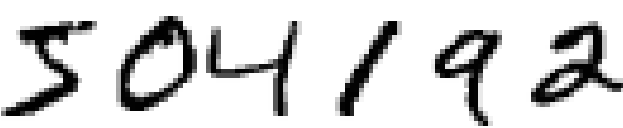
\includegraphics[scale=0.7]{figures/digits}
%\caption{\small \sl Figuren viser tallene 504192. \cite{Nielsen 2019} \label{fig:digits}} 
%\end{center} 
%\end{figure} 

%Menneskets evne til å se er en av de mest fasinerende mirakelene i naturen. Folk flest kan uten anstrengelse gjenkjenne tallene 504192 i figur \ref{fig:digits}. At dette er lett er et under, og ikke minst misledende. In each hemisphere of our brain, humans have a primary visual cortex, also known as V1, containing 140 million neurons, with tens of billions of connections between them. And yet human vision involves not just V1, but an entire series of visual cortices - V2, V3, V4, and V5 - doing progressively more complex image processing. We carry in our heads a supercomputer, tuned by evolution over hundreds of millions of years, and superbly adapted to understand the visual world. Recognizing handwritten digits isn't easy. Rather, we humans are stupendously, astoundingly good at making sense of what our eyes show us. But nearly all that work is done unconsciously. And so we don't usually appreciate how tough a problem our visual systems solve.

%The difficulty of visual pattern recognition becomes apparent if you attempt to write a computer program to recognize digits like those above. What seems easy when we do it ourselves suddenly becomes extremely difficult. Simple intuitions about how we recognize shapes - "a 9 has a loop at the top, and a vertical stroke in the bottom right" - turn out to be not so simple to express algorithmically. When you try to make such rules precise, you quickly get lost in a morass of exceptions and caveats and special cases. It seems hopeless.

%Neural networks approach the problem in a different way. The idea is to take a large number of handwritten digits, known as training examples

\subsubsection{Objektdeteksjon}

Objektdeteksjon handler om to ting. Områder av bilde som kan inneholde en klasse må genereres, og så må disse delene av et bilde klassifiseres basert på det visuelle innholdet i bildeområdet, et bildeområde kalles for en $patch$ innenfor maskinsyn \cite{LeCun m.fl. 1998 s. 23}. Områdene der det kan være objekter kalles for ankre. Med andre ord, målet for modellen er å se på en del av et bilde og finne ut hvilket objekt som finnes i dette området. Nettverket kan kun finne de objektene som den har blitt trent til å gjenkjenne.

\subsubsection{Dataaugmentering}

Dataen som skal brukes til å trene en maskinlæringsmodell må først normaliseres på en standard måte, for eksempel ved å subtrahere gjennomsnittet over dataen, for så å skalere alle bildene slik at de får samme størrelse. Dette gjør at nettverket kan trenes på data med ulike oppløsninger. Det er også mulig å gjøre flere andre endringer. Støy kan legges til bildene, samt å snu dem horisontalt eller vertikalt for å skape nye bilder å trene nettverket på. \cite{Cadieu m.fl. 2014 s. 15}

\subsubsection{Heterogene maskiner}

%Alle datamaskiner er i dag heterogene. De består av en CPU og en GPU, en Central Processing Unit og en Graphics Processing Unit. GPU-en kommer fra dataspillindustrien. Den første personlige datamaskinen, Apple ][, som var en kopi av spillmaskinen Atari 2600, hadde ikke en GPU. Etter Star Fox fra Argonaut Software, 1993, som var et spill som inneholdt den første GPU-en, så begynte flere maskiner å inkludere GPU-er.\footnote{Google viser sin respekt til den første GPU-en SuperFX som var i StarFox. Skriv «Do a barrel roll», en kjent replikk fra spillet, inn i google og se nettsiden rulle rundt y-aksen} På personlige datamaskiner og mobiltelefoner så har GPU-en gjort at maskinene bruker mindre strøm, som har ført til bedre batterilevetid. Datamaskiner, slik forbrukere typisk forstår dem, er inspirert av Xerox Alto, sekretærens datamaskin. I dag programmerer mange mennesker maskiner ved å ta i bruk grafiske brukergrensesnitt, og gjør arbeidet som tidligere var gjort av sekretærer. Alt fra regneark, skrive på maskin, telefonsamtaler osv. gjøres pliktoppfyllende på et digitalt skrivebord. Hver av disse maskinene, telefon, skrivemaskin, kalkulator, er ikke lenger på pulten til dagens sekretærer, de har blitt ikoner i et grafisk brukergrensesnitt. Dette hadde ikke vært mulig uten Atari og deres innovasjoner som gjorde sanntids-grafikk på billig maskinvare mulig.

Alle datamaskiner er i dag heterogene. De består av en CPU og en GPU, en Central Processing Unit og en Graphics Processing Unit. En programmerer CPU-en med språk slik som Python, C, C++, osv. Til å begynne med så var grafikkprosessorer fixed-function, et bestemt API tillot maskinvareakselerasjon av enkelte grafikkinstrukser. \cite{Buck 2006 s. 5}

I 2006 introduserte Nvidia den første generelt programmerbare GPU-en, deres nye grafikkprosessorer kunne programmeres i CUDA, et språk som ligner på C. Dette gjorde det mulig å gjøre andre ting enn grafikk på grafikkprosessorer. Grafikkprosessorer er spesielt flinke til oppgaver som er «massively parallell». \cite{Buck 2006 s. 1} %Forskere begynte å simulere proteiner og celler på GPU-en, det finnes for eksempel et prosjekt som heter Folding@home, der forbrukere kan låne bort GPU-en sin til forskning. Proteiner som fører til sykdommer slik som COVID-19 og parkinsons sykdom blir forsøkt forstått ved å gjøre simulasjoner på maskinene hjemme hos folk, forskningen krever enorme mengder datakraft.

\begin{figure}[t]
\begin{center} 
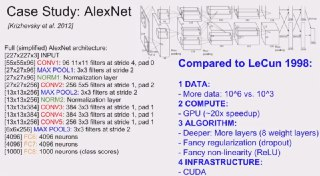
\includegraphics[scale=1.0]{figures/comparison}
\caption{\small \sl Figuren viser AlexNet på venstre side, og nye fremskritt på høyre side som har gjort deep learning populært. \cite{Karpathy 2014} \label{fig:comparison}}
\end{center} 
\end{figure} 

Det er ikke tilfeldig at det var i 2012 at deep learning tok av. Alex sitt team anvendte CUDA til å gjøre maskinlæring på en GPU istedet for en CPU, det hadde ikke blitt gjort tidligere \cite{Krizhevsky m.fl. 2012}. De anvendte en ikke-lineær aktiveringsfunksjon, noe som hadde blitt oppfunnet relativt nylig \cite{LeCun m.fl. 1998 s. 3}. Resultatene har ført til en revolusjon innenfor kunstig intelligens. Batch normalization har også forbedret resultatene. Se figur \ref{fig:comparison}. \cite{Ioffe og Szegedy 2015 s. 1}

I dette forsøket ble en GPU anvendt til å gjøre maskinlæring, å trene deep learning-modeller.

\subsubsection{Maskinlæringsrammeverk}

Det har blitt utviklet flere maskinlæringsrammeverk. Disse reduserer mye av kompleksiteten som går med på å lage nye modeller, og å trene modeller med ny data. Rammeverkene gjør at en får maskinvareakselerasjon av backpropagation og andre maskinlæringsutregninger uten at en trenger å lære seg CUDA. I dette forsøket ble Detectron2 med rammeverket PyTorch og YOLO med rammeverket Darknet anvendt til objektdeteksjon. Se figur \ref{fig:dl_libs}.

\begin{figure}[t]
\begin{center} 

\includegraphics[scale=0.30]{figures/darknet-logo}

\includegraphics[scale=0.30]{figures/Pytorch_logo}
\caption{\small \sl Figuren viser logoene til Darknet og PyTorch. Darknet er et populært rammeverk for maskinlæring skrevet i C \cite{Redmon 2016}. PyTorch er maskinlæringsrammeverk fra facebook, den anvendes av objektdeteksjonssystemet detectron2 \cite{Wu m.fl. 2020}. \label{fig:dl_libs}}
\end{center} 
\end{figure} 

\subsubsection{Azure nettsky}

En virtuell maskin med en GPU ble leid fra nettskytjenesten Azure fra Microsoft til å trene modellene i dette forsøket. Satya Mallick presenterer hvordan en lager en virtuell maskin på nettskytjenesten Azure i kurset Deep Learning with PyTorch. Du kan lage virtuelle maskiner fra Azure Portal. Å begynne med Deep Learning er superenkelt med Azure. Azure gir deg virtuelle instanser med nesten alle de mest populære deep learning-rammeverkene ferdiginstallert på deres Data Science Virtual Machines. Da slipper man å bruke tid på installering av Nvidia-drivere og andre deep learning-biblioteker. Maskinene kommer også med JupyterHub ferdig installert, om en ønsker å anvende Jupyter Notebooks. \cite{Mallick m.fl. 2020}

%Se vedlegg \ref{appendix:azure} for instrukser om hvordan man lager en Data Science Virtual Machine instanse med Ubuntu Linux 18.04 på Azure.

\subsubsection{SSH login}

SSH ble anvendt til å logge inn i den GPU-akselererte nettskyinstansen. SSH er et dataprogram og protokoll som anvendes til å koble til eksterne maskiner. Den er først og fremst rettet mot Unix-maskiner, og har et tekstgrensesnitt \cite{Mallick m.fl. 2020}. På Windows så kan dataprogrammet PuTTY anvendes\footnote{\url{https://www.putty.org/}}.

Etter at systemet på Azure er oppe så kan man logge inn.%, se vedlegg \ref{appendix:ssh} for en guide til SSH.%Once your system is up, the first thing that comes to your mind is how do I get in? We will see the steps involved in logging in to your system using SSH.

Å leie en GPU kan bli dyrt. Ikke glem å stoppe den virtuelle maskinen når den ikke er i bruk. Dette kan gjøres fra portalen til Azure\footnote{\url{https://portal.azure.com}}.

%1. Get IP address
%Go to dashboard and click on the test-machine you created.

\subsubsection{Anaconda programvareutgivelse}

Python er et programmeringsspråk som er populært blant forskere\footnote{\url{https://www.kaggle.com/learn/python}}. \cite{Morris 2020}

Anaconda er en programvareutgivelse som gjør det enkelt å bruke Python. Anaconda er også veldig nyttig for å unngå pakkekonflikter. På en Azure Data Science Virtual Machine så kommer flere Anaconda-miljøer ferdiginstallert. Anaconda PyTorch kan aktiveres med kommandoen \texttt{conda activate py37\_pytorch}. \cite{Mallick m.fl. 2020} %Se vedlegg \ref{appendix:ssh} for en guide til SSH der Anaconda blir anvendt til å aktivere et Python 3 miljø.

\subsubsection{Label-data}

Label-data er informasjon som beskriver rådataen i et datasett. En modell må ha label-data for å forstå informasjonen i treningssettet. Å lage label-data er en vesentlig og tidskrevende del av treningen. Innholdet i rådataen bestemmer hva slags label-data som må lages. Å lage label-data kan gjøres manuelt eller automatisk av en maskin. Det kan gjøres in-house, eller bli gjort av forskjellige bedrifter. Om det er veldig mye data som må få label-data så kan prosessen bli svært tidskrevende og dyrt. \cite{Kaller 2019}


\subsubsection{RetinaNet}

RetinaNet, introdusert av Facebook-ansatte i 2017 i Focal Loss for Dense Object Detection på arXiv, ble ansett som den beste objektdeteksjonsmodellen da dette dokumentet ble skrevet. Det var en forbedring av R-CNN. \cite{Lin m.fl. 2017}

RetinaNet er implementert i Detectron2, som bruker deep learning-rammeverket PyTorch. Grensesnittet er programmeringsspråket Python 3. Detectron2 er utgitt under en Apache 2.0-lisens, det vil si at den kan brukes til hva enn en vil på en hvilken som helst måte, gratis, så lenge man aksepterer at Facebook ikke blir ansvarlig for arbeidet som gjøres, og så lenge man ikke krediterer arbeidet en gjør til Facebook \cite{The Apache Software Foundation 2004}. Detectron2 installeringsinstrukser er tilgjengelig på nettet.\footnote{\url{https://detectron2.readthedocs.io/}}

\subsubsection{YOLO}

You only look once (YOLO) er en state-of-the-art, real-time objektdeteksjonssystem. På en Pascal Titan X, en mektig Nvidia-GPU, så prosesserer den bilder ved 30 FPS og har en mAP på 57.9 \% på COCO test-dev \cite{Redmon 2018}. På min Macbook Pro fra 2017 så drar den 1 FPS på CPU-en på datasettet presentert i denne oppgaven. Ifølge Redmon så er YOLO like bra som Focal Loss, det vil si RetinaNet, men omtrent fire ganger raskere. Redmon mener en kan lett endre størrelsen på YOLO modellen, den vil bli tregere men enda mer nøyaktig \cite{Redmon 2016}%. Se figur \ref{fig:yolo_inference}. % Se figur retinanet vs YOLOv4 resultater

\subsubsection{OpenCV}

OpenCV (Open Source Computer Vision Library) er et et programvarebibliotek for maskinsyn og maskinlæring med åpen kildekode. OpenCV ble laget for å levere en kjent infrastruktur for maskinsynprogrammer og OpenCV-teamet ønsker å gjøre maskinsensorikk mer utbredt i kommersielle produkter. OpenCV er et produkt gitt ut under BSD-lisensen, det gjør biblioteket tilgjengelig for bedrifter som ønsker å anvende kildekoden \cite{OpenCV Team 2020}.

OpenCV har grensesnitt for C++, Python, Java og MATLAB og støtter Windows, Linux, Android og macOS. OpenCV-teamet forsøker først og fremst å levere sanntids maskinsyn for dataprogrammer og drar nytte av prosessorteknologi slik som MMX- og SSE-instruksjoner når de er tilgjengelige. Støtte for CUDA og OpenCL var under utvikling, men var enda ikke tilgjengelig da denne oppgaven ble skrevet. Det hadde gjort dataprogrammet mye raskere siden den ville dratt nytte av GPU-en og ikke bare CPU-en på maskinen. OpenCV er skrevet i C++ og virker uten navnekonflikter med STL namespaces. \cite{OpenCV Team 2020}

\subsection{Tidligere arbeid}

\label{part:prev_work}
Noen forskere har allerede rukket å anvende «deep learning» til å klassifisere fisk fra undervannsvideo. I 2016 presenterte CVG Jena Fulda teamet resultater av klassifisering av fisk på SeaCLEF-datasettet. De anvendte «convolutional» nevrale nettverk, nettverk for bildeklassifisering, og klarte å gjøre objektdeteksjon samt å klassifisere forskjellige fiskearter. De testet bakgrunnssubtraksjon, en teknikk som var typisk for deteksjon av objekter i undervannsbilder på den tiden. De fant ut at å bruke bakgrunnssubtraksjon fungerte dårligere enn «object proposal classification» (OPC) for deteksjon av fisk. \cite{Rodner m.fl. 2016}

%En interessant referanse som kan tas med under tidligere arbeid er Deep Vision-systemet som har vært testet av Havforskningsinstituttet: https://www.tu.no/artikler/na-kan-maskinen-skille-mellom-makrell-og-sild/464208?utm_source=newsletter-tudaily&utm_medium=email&utm_campaign=newsletter-2019-05-06.

Også i Norge så har det blitt gjort forsøk på maskinsyn og maskinlæring innenfor havforskning. Havforskningsinstituttet testet ut Deep Vision, et kamerasystem fra Scantrol Deep Vision AS, i 2017, 2018 og senest igjen i 2019. Kamerasystemet ble festet ved inngangen til en trål for å måle mengde og artsbestemme fisk uten å hente den om bord og ta livet av den. Poenget med maskinlæringen var å automatisere artsbestemmelsen. Artsbestemmelsen ble gjort tidligere ved at forskere tolker hvert bilde kameraene tar manuelt. Modellen til Scantrol Deep Vision kunne gjenkjenne artene sild, kolmule, makrell og lysprikkfisk. Forsøkene viste at omtrent 90 prosent av fisken ble riktig identifisert av systemet. \cite{Fenstad 2019}

Det norske kompaniet Skala Maskon har også sett på maskinsyn, de har utviklet en vaksineringsmaskin som bruker maskinsyn for å finne punktet hvor vaksinen skal settes på hver fisk. De bruker programvare fra Scorpion Vision. Skala Maskons fullautomatiske vaksinemaskin drives av en enkelt operatør og kan vaksinere og sortere opp til 40 000 smolt i timen. Maskinene kan vaksinere singel, dobbel, trippel og intramuskulære doser samtidig. \cite{Falstad 2016}

Siddiqui sitt team presenterte i 2017 klassifisering av forskjellige fiskearter i undervannsvideoer der de brukte en modell med vekter fra forhåndstrente dype nettverk. Det er et eksempel på såkalt «transfer learning». Dette automatiske systemet kunne med høy nøyaktighet detektere, tracke og klassifisere fisk og andre marine arter i undervannsvideoer uten menneskelig overvåkning. De oppdaget at typiske maskinsynteknikker fungerer dårlig på undervannsbilder. Bakgrunnen er kompleks og både fasongen og teksturen på de forskjellige fiskeartene kan være svært like. Datadrevne programmer, slik som nevrale nettverk, krever enorme mengder kategorisert data, ellers har de en tendens til å overtilpasse treningsdataen og feiler når den blir gitt testdata som den ikke har sett før, det vil si data som ble utelatt ved treningen. I artikkelen deres  «Automatic fish species classification in underwater videos» presenteres state-of-the-art maskinsynsmetoder for fine-grained klassifisering av fiskearter basert på deep learning teknikker. Konvolveringsnettverk, nettverkene som anvendes til bildeklassifisering, ble forhåndstrent på et mye større og mer generelt datasett. Ved å forhåndstrene nettverket på et generelt datasett så kan man bruke mindre treningsdata. SVM ble brukt til å trene nettverket og de oppnådde en nøyaktighet på 94.3 \%. De tropiske fiskeartene ble tatt fra undervannsvideoer fra kysten av vest-Australia. Forskerne mener automatiske klassifiseringssystemer kan brukes til å identifisere fisk fra undervannsvideoer, og at det er et billig alternativ til manuell identifikasjon av fisk. \cite{Siddiqui m.fl. 2017}

\begin{figure}
\begin{center} 
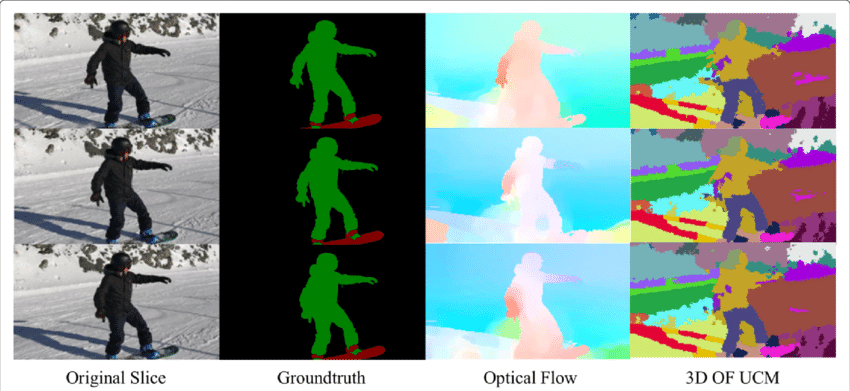
\includegraphics[scale=0.45]{figures/optical_flow}
\caption{\small \sl Figuren viser semantisk segmentering generert fra optical flow. Optical flow er bevegelsene av objektene mellom bildene i en film. \cite{Lin 2019}
\label{fig:optical_flow}} 
\end{center} 
\end{figure} 

I 2018 presenterte Xu og Matzner forskning på deteksjon, tracking og klassifisering av fisk i undervannsvideoer. Undervannsvideoer anvendes til å studere økosystemene i havene og i elver, først og fremst for å drive med miljøforskning. Å observere mengden av liv, samt vanene til fiskene i forskjellige miljø, er eksempler på miljøforskning. Optisk video gir detaljert informasjon som mennesker kan forstå. Mennesker kan naturlig forstå verden visuelt, men manuell analyse av video tar tid. Å automatisere arbeidet er nødvendig om en har store datamengder, og en ønsker å få arbeidet fullført på en gitt tid på en effektiv måte. Dette kan være nødvendig om en skal gjøre gode avgjørelser som påvirker de marine økosystemene. Maskinsyn og maskinlæring har vist seg å være effektive metoder for å automatisere overvåking. Undervannsbilder er kjent for å være spesielt utfordrende å håndtere. Mengden lys under vann varierer over tid, og mengden lys påvirkes også av avstand fra lyskilder. Det er lite kontrast under vann og bakgrunnen er ofte svært avansert, den består av blant annet flytende vegetasjon. Videre påvirkes bildene av turbiditet. \cite{Xu og Matzner 2018}

%Skala Maskon (https://www.skalamaskon.no/) har utviklet en vaksineringsmaskin som bruker maskinsyn for å finne punktet hvor vaksinen skal settes på hver fisk. De bruker programvare fra Scorpion Vision (http://www.scorpionvision.com/).

Salman sitt team viste i 2019 at de kunne estimere biomasse automatisk ved å bruke undervannsvideoer og dype nevrale nettverk.  Et slikt system må takle varierende lysstyrke, vinkelen fiskene sees fra, forskjellige havbunnsstrukturer, bevegelser i vegetasjon i bakgrunnen og forskjellige former og teksturer mellom fiskearter. De anvendte en Region-Based Convolutional Neural Network, et R-CNN, som er en state-of-the-art maskinlæringsteknikk, et alternativ til YOLO. Teknologien anvendes til objektdeteksjon, den gir informasjon om hvor i et bilde forskjellige objekter er samt hvor mange det er av de forskjellige objektene. De trente et nettverk og anvendte bakgrunnssubtraksjon og optical flow, sammen med råbilde ga dette områder der fisk skulle detekteres. Optical flow er bevegelsen av objektene mellom fortløpende bilder i en sekvens, det kommer av de relative bevegelsene mellom objektet og kameraet. Det brukes til bildesegmentering \cite{Lin 2019}. Se figur \ref{fig:optical_flow}. De brukte to datasett, et fra Fish4Knowledge sitt Complex Scenes-datasett, den består av undervannsvideoer, og LifeCLEF 2015-datasettet. Resultatene de fikk var så gode at de anbefaler teknikkene som de har anvendt for fiskedeteksjon til andre med lignende problemer. \cite{Salman m.fl. 2019}

\begin{figure}
\begin{center} 
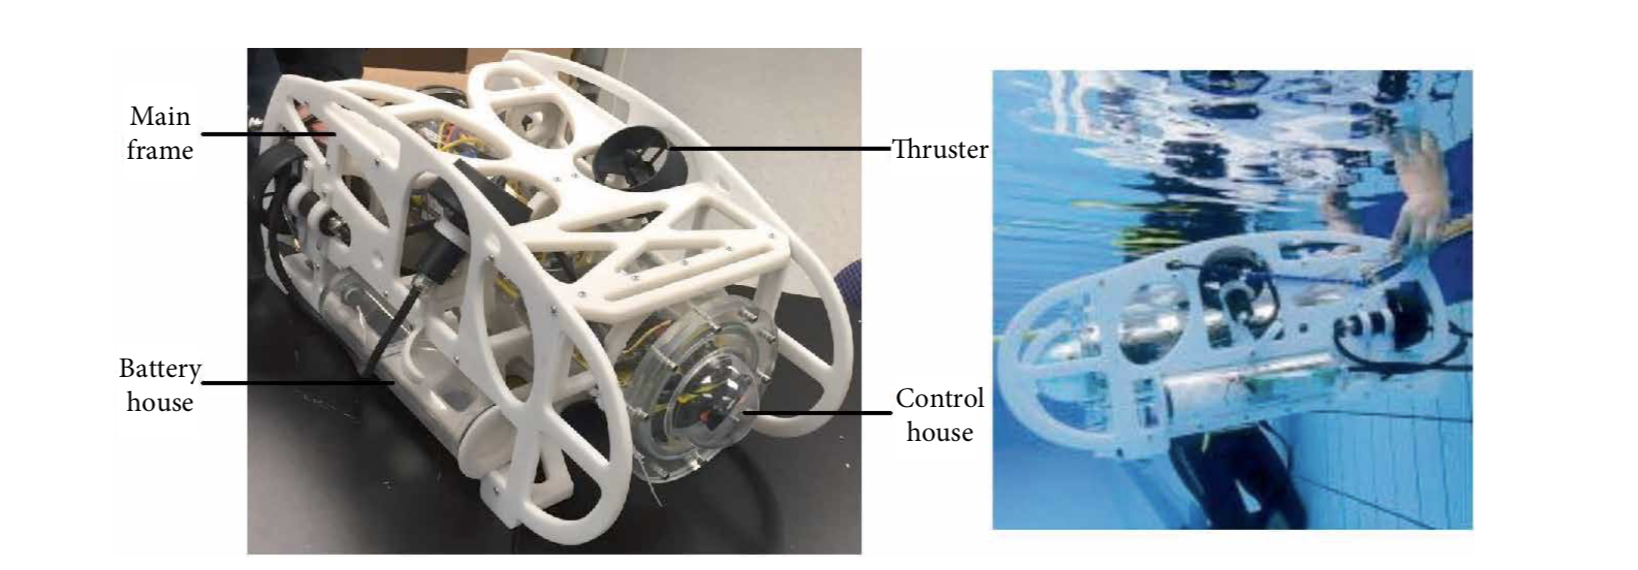
\includegraphics[scale=0.45]{figures/auv}
\caption{\small \sl Figuren viser roboten til Cui sitt team. Den kan detektere fisk og skal brukes til havforskning. \cite{Cui m.fl. 2020} \label{fig:auv}} 
\end{center} 
\end{figure} 

I 2020 så skrev Cui sitt team «Fish Detection Using Deep Learning». De jobber på en robot som kan utforske havet, se figur \ref{fig:auv}. I artikkelen deres dokumenterer de hvordan en lager en modell, et nevralt nettverk, som kan utføre fiskedeteksjon. De anvendte «data augmentation»-teknikker. De brukte også Dropout-algoritmen for å hindre at modellen ble overtilpasset, kjent som «overfitting»-problemet. De endret også på loss-funksjonen ettersom nettverket ble trent. Ved å bruke disse teknikkene så klarte de å redusere treningstiden og training loss. Systemet de lagde var optimalisert for et innebygd system, altså en svakere datamaskin, en AUV-robot. \cite{Cui m.fl. 2020}

%\subsection{Perceptron}

%\subsection{Sigmoid neurons}




%Deep learning and unsupervised feature learning have shown great promise in many practical ap- plications. State-of-the-art performance has been reported in several domains, ranging from speech recognition [1, 2], visual object recognition [3, 4], to text processing [5, 6].

%It has also been observed that increasing the scale of deep learning, with respect to the number of training examples, the number of model parameters, or both, can drastically improve ultimate classification accuracy [3, 4, 7]. These results have led to a surge of interest in scaling up the training and inference algorithms used for these models [8] and in improving applicable optimization procedures [7, 9]. The use of GPUs [1, 2, 3, 8] is a significant advance in recent years that makes the training of modestly sized deep networks practical. A known limitation of the GPU approach is that the training speed-up is small when the model does not fit in GPU memory (typically less than 6 gigabytes). To use a GPU effectively, researchers often reduce the size of the data or parameters so that CPU-to-GPU transfers are not a significant bottleneck. While data and parameter reduction work well for small problems (e.g. acoustic modeling for speech recognition), they are less attractive for problems with a large number of examples and dimensions (e.g., high-resolution images).

%\subsection{Maskinlæring}

%Over the last several years􏰈 machine learning techniques􏰈 particularly when applied to neural networks􏰈 have played an increasingly imp ortant role in the design of pattern recognition systems􏰇 In fact􏰈 it could be argued that the availability of learning techniques has b een a crucial fac􏰗 tor in the recent success of pattern recognition applications such as continuous speech recognition and handwriting recognition.

%\subsubsection{Data is king}
%\subsubsection{Datainnsamling}
%\subsection{Modell}
%\subsubsection{Den biologiske inspirasjonen}
%\subsubsection{Bias}
%\subsection{Algoritme}
%\subsection{Objektdeteksjon}

%Our core visual processing module is a Convolutional Neural Network (CNN) [29, 26], which has emerged as a powerful model for visual recognition tasks [38]. The first application of these models to dense predic- tion tasks was introduced in R-CNN [15], where each re- gion of interest was processed independently. Further work has focused on processing all regions with only single for- ward pass of the CNN [18, 14], and on eliminating explicit region proposal methods by directly predicting the bound- ing boxes either in the image coordinate system [45, 10], or in a fully convolutional [31] and hence position-invariant settings [39, 37, 36]. Most related to our approach is the work of Ren et al. [37] who develop a region proposal net- work (RPN) that regresses from anchors to regions of in- terest. However, they adopt a 4-step optimization process, while our approach does not require training pipelines. Ad- ditionally, we replace their RoI pooling mechanism with a differentiable, spatial soft attention mechanism [20, 17]. In particular, this change allows us to backpropagate through the region proposal network and train the whole model jointly.

%\subsection{Trening}
%\subsection{Evaluering}
%\subsubsection{Nøyaktighet} % error rate
%\subsubsection{Presisjon} 
%\subsubsection{Konfidensintervall} % confidence interval
%\subsection{Inferens}
%\subsubsection{Ground truth} %(grunnfestet sanhet?)
%\subsubsection{Bilder per sekund} %FPS (bilder per sekund)
%\subsubsection{State-of-the-art maskinsyn} % (topp moderne)
%\subsubsection{Real-time} %(sanntid)
%\subsection{Segmentering}

%Machine Learning: Learning from data
%
%Data is king.
%
%Data collection, annotation, preporation etc.
%
%Data > Algorithm > Training > Evaluation > Deployment > Predictions
%
%	Gather data from every legal source possible (public data sets, purchase data, collect data, synthesize data (super poweful))
%
%	Manually check data
%	Look for biases
%	Look for insights
%	Clean up
%
%	Iterative: Partition data 60 (training)/20 (testing accuracy training)/20 (test)
%
%Model / Algorithm
%
%	Image classification
%	Object detection
%	Segmentation
%
%	Constraints
%
%	Experimentation (test multiple viable models)
%
%Training
%
%	Data augmentation
%	Training parameter (optimizer, rate etc.)
%	Visualizsation (check if it is going correctly)
%
%Evaluation
%
%	Test. Check model size, speed and ACCURACY
%
%Deployment
%
%	Optimizations, deploy, feedback (know when it went badly, check failed images)
%
%\subsection{Build your own}
%
%Build your own:
%
%1) Pick a state-of-the-art architecture
%
%2) Make sure there is an open-source implementation
%
%3) Make sure you get weights for this network trained on ImageNet
%
%
%Experiment
%
%1) Minimal architectural change
%	Fine tune
%
%2) If not enough: Tweak architecture
%	More network blocks, new types of layers etc.
%
%3) Search (Google's neural architecture search)
%
%\subsection{resnet}
%
%\begin{comment}
%ResNet(
%  (conv1): Conv2d(3, 64, kernel_size=(7, 7), stride=(2, 2), padding=(3, 3), bias=False)
%  (bn1): BatchNorm2d(64, eps=1e-05, momentum=0.1, affine=True, track_running_stats=True)
%  (relu): ReLU(inplace=True)
%  (maxpool): MaxPool2d(kernel_size=3, stride=2, padding=1, dilation=1, ceil_mode=False)
%  (layer1): Sequential(
%    (0): Bottleneck(
%      (conv1): Conv2d(64, 64, kernel_size=(1, 1), stride=(1, 1), bias=False)
%      (bn1): BatchNorm2d(64, eps=1e-05, momentum=0.1, affine=True, track_running_stats=True)
%      (conv2): Conv2d(64, 64, kernel_size=(3, 3), stride=(1, 1), padding=(1, 1), bias=False)
%      (bn2): BatchNorm2d(64, eps=1e-05, momentum=0.1, affine=True, track_running_stats=True)
%      (conv3): Conv2d(64, 256, kernel_size=(1, 1), stride=(1, 1), bias=False)
%      (bn3): BatchNorm2d(256, eps=1e-05, momentum=0.1, affine=True, track_running_stats=True)
%      (relu): ReLU(inplace=True)
%      (downsample): Sequential(
%        (0): Conv2d(64, 256, kernel_size=(1, 1), stride=(1, 1), bias=False)
%        (1): BatchNorm2d(256, eps=1e-05, momentum=0.1, affine=True, track_running_stats=True)
%      )
%    )
%    (1): Bottleneck(
%      (conv1): Conv2d(256, 64, kernel_size=(1, 1), stride=(1, 1), bias=False)
%      (bn1): BatchNorm2d(64, eps=1e-05, momentum=0.1, affine=True, track_running_stats=True)
%      (conv2): Conv2d(64, 64, kernel_size=(3, 3), stride=(1, 1), padding=(1, 1), bias=False)
%      (bn2): BatchNorm2d(64, eps=1e-05, momentum=0.1, affine=True, track_running_stats=True)
%      (conv3): Conv2d(64, 256, kernel_size=(1, 1), stride=(1, 1), bias=False)
%      (bn3): BatchNorm2d(256, eps=1e-05, momentum=0.1, affine=True, track_running_stats=True)
%      (relu): ReLU(inplace=True)
%    )
%    (2): Bottleneck(
%      (conv1): Conv2d(256, 64, kernel_size=(1, 1), stride=(1, 1), bias=False)
%      (bn1): BatchNorm2d(64, eps=1e-05, momentum=0.1, affine=True, track_running_stats=True)
%      (conv2): Conv2d(64, 64, kernel_size=(3, 3), stride=(1, 1), padding=(1, 1), bias=False)
%      (bn2): BatchNorm2d(64, eps=1e-05, momentum=0.1, affine=True, track_running_stats=True)
%      (conv3): Conv2d(64, 256, kernel_size=(1, 1), stride=(1, 1), bias=False)
%      (bn3): BatchNorm2d(256, eps=1e-05, momentum=0.1, affine=True, track_running_stats=True)
%      (relu): ReLU(inplace=True)
%    )
%  )
%  (layer2): Sequential(
%    (0): Bottleneck(
%      (conv1): Conv2d(256, 128, kernel_size=(1, 1), stride=(1, 1), bias=False)
%      (bn1): BatchNorm2d(128, eps=1e-05, momentum=0.1, affine=True, track_running_stats=True)
%      (conv2): Conv2d(128, 128, kernel_size=(3, 3), stride=(2, 2), padding=(1, 1), bias=False)
%      (bn2): BatchNorm2d(128, eps=1e-05, momentum=0.1, affine=True, track_running_stats=True)
%      (conv3): Conv2d(128, 512, kernel_size=(1, 1), stride=(1, 1), bias=False)
%      (bn3): BatchNorm2d(512, eps=1e-05, momentum=0.1, affine=True, track_running_stats=True)
%      (relu): ReLU(inplace=True)
%      (downsample): Sequential(
%        (0): Conv2d(256, 512, kernel_size=(1, 1), stride=(2, 2), bias=False)
%        (1): BatchNorm2d(512, eps=1e-05, momentum=0.1, affine=True, track_running_stats=True)
%      )
%    )
%    (1): Bottleneck(
%      (conv1): Conv2d(512, 128, kernel_size=(1, 1), stride=(1, 1), bias=False)
%      (bn1): BatchNorm2d(128, eps=1e-05, momentum=0.1, affine=True, track_running_stats=True)
%      (conv2): Conv2d(128, 128, kernel_size=(3, 3), stride=(1, 1), padding=(1, 1), bias=False)
%      (bn2): BatchNorm2d(128, eps=1e-05, momentum=0.1, affine=True, track_running_stats=True)
%      (conv3): Conv2d(128, 512, kernel_size=(1, 1), stride=(1, 1), bias=False)
%      (bn3): BatchNorm2d(512, eps=1e-05, momentum=0.1, affine=True, track_running_stats=True)
%      (relu): ReLU(inplace=True)
%    )
%    (2): Bottleneck(
%      (conv1): Conv2d(512, 128, kernel_size=(1, 1), stride=(1, 1), bias=False)
%      (bn1): BatchNorm2d(128, eps=1e-05, momentum=0.1, affine=True, track_running_stats=True)
%      (conv2): Conv2d(128, 128, kernel_size=(3, 3), stride=(1, 1), padding=(1, 1), bias=False)
%      (bn2): BatchNorm2d(128, eps=1e-05, momentum=0.1, affine=True, track_running_stats=True)
%      (conv3): Conv2d(128, 512, kernel_size=(1, 1), stride=(1, 1), bias=False)
%      (bn3): BatchNorm2d(512, eps=1e-05, momentum=0.1, affine=True, track_running_stats=True)
%      (relu): ReLU(inplace=True)
%    )
%    (3): Bottleneck(
%      (conv1): Conv2d(512, 128, kernel_size=(1, 1), stride=(1, 1), bias=False)
%      (bn1): BatchNorm2d(128, eps=1e-05, momentum=0.1, affine=True, track_running_stats=True)
%      (conv2): Conv2d(128, 128, kernel_size=(3, 3), stride=(1, 1), padding=(1, 1), bias=False)
%      (bn2): BatchNorm2d(128, eps=1e-05, momentum=0.1, affine=True, track_running_stats=True)
%      (conv3): Conv2d(128, 512, kernel_size=(1, 1), stride=(1, 1), bias=False)
%      (bn3): BatchNorm2d(512, eps=1e-05, momentum=0.1, affine=True, track_running_stats=True)
%      (relu): ReLU(inplace=True)
%    )
%  )
%  (layer3): Sequential(
%    (0): Bottleneck(
%      (conv1): Conv2d(512, 256, kernel_size=(1, 1), stride=(1, 1), bias=False)
%      (bn1): BatchNorm2d(256, eps=1e-05, momentum=0.1, affine=True, track_running_stats=True)
%      (conv2): Conv2d(256, 256, kernel_size=(3, 3), stride=(2, 2), padding=(1, 1), bias=False)
%      (bn2): BatchNorm2d(256, eps=1e-05, momentum=0.1, affine=True, track_running_stats=True)
%      (conv3): Conv2d(256, 1024, kernel_size=(1, 1), stride=(1, 1), bias=False)
%      (bn3): BatchNorm2d(1024, eps=1e-05, momentum=0.1, affine=True, track_running_stats=True)
%      (relu): ReLU(inplace=True)
%      (downsample): Sequential(
%        (0): Conv2d(512, 1024, kernel_size=(1, 1), stride=(2, 2), bias=False)
%        (1): BatchNorm2d(1024, eps=1e-05, momentum=0.1, affine=True, track_running_stats=True)
%      )
%    )
%    (1): Bottleneck(
%      (conv1): Conv2d(1024, 256, kernel_size=(1, 1), stride=(1, 1), bias=False)
%      (bn1): BatchNorm2d(256, eps=1e-05, momentum=0.1, affine=True, track_running_stats=True)
%      (conv2): Conv2d(256, 256, kernel_size=(3, 3), stride=(1, 1), padding=(1, 1), bias=False)
%      (bn2): BatchNorm2d(256, eps=1e-05, momentum=0.1, affine=True, track_running_stats=True)
%      (conv3): Conv2d(256, 1024, kernel_size=(1, 1), stride=(1, 1), bias=False)
%      (bn3): BatchNorm2d(1024, eps=1e-05, momentum=0.1, affine=True, track_running_stats=True)
%      (relu): ReLU(inplace=True)
%    )
%    (2): Bottleneck(
%      (conv1): Conv2d(1024, 256, kernel_size=(1, 1), stride=(1, 1), bias=False)
%      (bn1): BatchNorm2d(256, eps=1e-05, momentum=0.1, affine=True, track_running_stats=True)
%      (conv2): Conv2d(256, 256, kernel_size=(3, 3), stride=(1, 1), padding=(1, 1), bias=False)
%      (bn2): BatchNorm2d(256, eps=1e-05, momentum=0.1, affine=True, track_running_stats=True)
%      (conv3): Conv2d(256, 1024, kernel_size=(1, 1), stride=(1, 1), bias=False)
%      (bn3): BatchNorm2d(1024, eps=1e-05, momentum=0.1, affine=True, track_running_stats=True)
%      (relu): ReLU(inplace=True)
%    )
%    (3): Bottleneck(
%      (conv1): Conv2d(1024, 256, kernel_size=(1, 1), stride=(1, 1), bias=False)
%      (bn1): BatchNorm2d(256, eps=1e-05, momentum=0.1, affine=True, track_running_stats=True)
%      (conv2): Conv2d(256, 256, kernel_size=(3, 3), stride=(1, 1), padding=(1, 1), bias=False)
%      (bn2): BatchNorm2d(256, eps=1e-05, momentum=0.1, affine=True, track_running_stats=True)
%      (conv3): Conv2d(256, 1024, kernel_size=(1, 1), stride=(1, 1), bias=False)
%      (bn3): BatchNorm2d(1024, eps=1e-05, momentum=0.1, affine=True, track_running_stats=True)
%      (relu): ReLU(inplace=True)
%    )
%    (4): Bottleneck(
%      (conv1): Conv2d(1024, 256, kernel_size=(1, 1), stride=(1, 1), bias=False)
%      (bn1): BatchNorm2d(256, eps=1e-05, momentum=0.1, affine=True, track_running_stats=True)
%      (conv2): Conv2d(256, 256, kernel_size=(3, 3), stride=(1, 1), padding=(1, 1), bias=False)
%      (bn2): BatchNorm2d(256, eps=1e-05, momentum=0.1, affine=True, track_running_stats=True)
%      (conv3): Conv2d(256, 1024, kernel_size=(1, 1), stride=(1, 1), bias=False)
%      (bn3): BatchNorm2d(1024, eps=1e-05, momentum=0.1, affine=True, track_running_stats=True)
%      (relu): ReLU(inplace=True)
%    )
%    (5): Bottleneck(
%      (conv1): Conv2d(1024, 256, kernel_size=(1, 1), stride=(1, 1), bias=False)
%      (bn1): BatchNorm2d(256, eps=1e-05, momentum=0.1, affine=True, track_running_stats=True)
%      (conv2): Conv2d(256, 256, kernel_size=(3, 3), stride=(1, 1), padding=(1, 1), bias=False)
%      (bn2): BatchNorm2d(256, eps=1e-05, momentum=0.1, affine=True, track_running_stats=True)
%      (conv3): Conv2d(256, 1024, kernel_size=(1, 1), stride=(1, 1), bias=False)
%      (bn3): BatchNorm2d(1024, eps=1e-05, momentum=0.1, affine=True, track_running_stats=True)
%      (relu): ReLU(inplace=True)
%    )
%  )
%  (layer4): Sequential(
%    (0): Bottleneck(
%      (conv1): Conv2d(1024, 512, kernel_size=(1, 1), stride=(1, 1), bias=False)
%      (bn1): BatchNorm2d(512, eps=1e-05, momentum=0.1, affine=True, track_running_stats=True)
%      (conv2): Conv2d(512, 512, kernel_size=(3, 3), stride=(2, 2), padding=(1, 1), bias=False)
%      (bn2): BatchNorm2d(512, eps=1e-05, momentum=0.1, affine=True, track_running_stats=True)
%      (conv3): Conv2d(512, 2048, kernel_size=(1, 1), stride=(1, 1), bias=False)
%      (bn3): BatchNorm2d(2048, eps=1e-05, momentum=0.1, affine=True, track_running_stats=True)
%      (relu): ReLU(inplace=True)
%      (downsample): Sequential(
%        (0): Conv2d(1024, 2048, kernel_size=(1, 1), stride=(2, 2), bias=False)
%        (1): BatchNorm2d(2048, eps=1e-05, momentum=0.1, affine=True, track_running_stats=True)
%      )
%    )
%    (1): Bottleneck(
%      (conv1): Conv2d(2048, 512, kernel_size=(1, 1), stride=(1, 1), bias=False)
%      (bn1): BatchNorm2d(512, eps=1e-05, momentum=0.1, affine=True, track_running_stats=True)
%      (conv2): Conv2d(512, 512, kernel_size=(3, 3), stride=(1, 1), padding=(1, 1), bias=False)
%      (bn2): BatchNorm2d(512, eps=1e-05, momentum=0.1, affine=True, track_running_stats=True)
%      (conv3): Conv2d(512, 2048, kernel_size=(1, 1), stride=(1, 1), bias=False)
%      (bn3): BatchNorm2d(2048, eps=1e-05, momentum=0.1, affine=True, track_running_stats=True)
%      (relu): ReLU(inplace=True)
%    )
%    (2): Bottleneck(
%      (conv1): Conv2d(2048, 512, kernel_size=(1, 1), stride=(1, 1), bias=False)
%      (bn1): BatchNorm2d(512, eps=1e-05, momentum=0.1, affine=True, track_running_stats=True)
%      (conv2): Conv2d(512, 512, kernel_size=(3, 3), stride=(1, 1), padding=(1, 1), bias=False)
%      (bn2): BatchNorm2d(512, eps=1e-05, momentum=0.1, affine=True, track_running_stats=True)
%      (conv3): Conv2d(512, 2048, kernel_size=(1, 1), stride=(1, 1), bias=False)
%      (bn3): BatchNorm2d(2048, eps=1e-05, momentum=0.1, affine=True, track_running_stats=True)
%      (relu): ReLU(inplace=True)
%    )
%  )
%  (avgpool): AdaptiveAvgPool2d(output_size=(1, 1))
%  (fc): Linear(in_features=2048, out_features=1000, bias=True)
%)
%\end{comment}
%\subsection{Andrej Karpathy}
%
%Andrej Karpathy (5,1 \%)
%
%% Generellt
%
%% Maskinsyn i matindustri
%
%% Mitt arbeid
%
%%Sjømatdivisjonen og Akvadivisjonen ved Nofima har en strategisk internsatsing\footnote{\url{https://nofima.no/prosjekt/sameksistens/}} som går ut på å samle kunnskap om sameksistens mellom ulike marine næringer og interesser, deriblant om hvordan man kan unngå konflikter mellom ulike interesser. 
%
%%En av problemstillingene er sameksistens mellom fiskeri- og oppdrettsnæringene, og hvordan oppdrettsanlegg påvirker de nærliggende fiskeplassene. I den forbindelse er det interessant å kartlegge omfanget av hvitfisk som beiter på fôr fra oppdrettsanlegg. Dette er en problemstilling som har vært i fokus hos media\footnote{For eksempel \url{https://fiskeribladet.no/nyheter/?artikkel=69867} (hentet 12.02.2020)} etter at flere fiskere har fanget fôrsprengt torsk og sei i fjorder hvor det finnes oppdrettsanlegg. Det hevdes at denne fisken er av betydelig dårligere kvalitet og den kan ha fått i seg medisiner gjennom fôret som gjør at den kan være farlig å spise. 
%
%%Det behøves kunnskap om hvor mange villfisk som trekker til oppdrettsanlegg, og under hvilke forhold, slik at man kan komme nærmere en løsning som kan dempe konflikten mellom disse to næringene. 
%
%%\subsection{Mål}
%
%%Målet med dette prosjektet er å utvikle et system som kan telle antall villfisk av ulike arter basert på en videostrøm fra et undervannskamera. Det er ønskelig å kunne vise resultatet som en fordeling av observasjoner over tid for hver art. 
%%Til dette prosjektet er det anskaffet et undervannskamera av typen Steinsvik Orbit-3300 som styres via et MB-3000 kontrollpanel. Dette systemet er utviklet for inspeksjon av fisk i merd og tar opp data i form av en analog videostrøm. Denne kan sendes gjennom en analog-digital-omformer til en datamaskin hvor dataene til slutt vil kunne prosesseres i sanntid. 
%
%%\subsection{Delmål}
%
%%\subsubsection{Programvare skrevet i C++}
%
%%Prosjektet består i hovedsak av å utvikle en programvare som kan gjøre følgende ved hjelp av maskinlæring: 
%
%%\begin{enumerate}
%%\item Segmentere fisk fra bakgrunn
%%\item Klassifisere hver fisk etter art
%%\item Spore hver fisk gjennom hvert bilde i videostrømmen inntil fisken forlater kameraets synsfelt
%%\end{enumerate}
%
%%Programvaren implementeres i C++ ved hjelp av OpenCV-biblioteket\footnote{https://opencv.org/}. Det kan også være aktuelt å lage et grafisk grensesnitt hvor tellingene fra hver art kan vises i sanntid, men dette er avhengig av om prosjektets omfang tillater det. 
%
%%\subsubsection{Praktisk del ved Havbruksstasjonen i Tromsø}
%
%%Det er planlagt en praktisk del hvor kameraet skal plasseres ut på oppdrettsanlegg og samle data som kan prosesseres i ettertid for å teste programvaren. Dette blir mest sannsynlig på Havbruksstasjonen i Tromsø. Å finne beste plasseringen av kameraet i forhold til merdene er en viktig del av dette arbeidet med tanke på synsfelt og lysforhold. 
%
%\subsubsection{Maskinsyn i matindustrien}
%
%Nofima is a research organisation in the food industry
%
%What about the salads and bama
%
%The mathematics course had both calculus and optimization
%
%You can explain about the tedious counting the salad leaves etc
%
%Your data camera may do this
%
%I can justify how computer vision is important in the food industry, and might revolutionize many industries
%
%I can say this is a problem Nofima has, and wanted it solved with computer vision, as it is not only done before it is also cheaper than getting someone to manually count fish.
%
%Say how you came to realise the importance doing practice at Bama, how you tried then to rig up a camera
%
%There are already several players
%
%You have marine robotics
%
%And you have StingRay
%
%The same with marine robotics
%
%They use OpenCV and Qt
%
%Mention that too lakselus very severe problem
%
%I could also mention solving problems in an interesting way is the difference between drudgery and fun
%
%And most problems are solved since they are interesting to someone
%
%%\section{Teori}
%
%\subsubsection{Introduksjon til kunstig intelligens}
%
%Dette er den offisielt første dagen av bacheloroppgaven. Den ble markert med en presentasjon av Sunniva Hoel, der hun presenterte blant annet innsida.ntnu.no/oppgaveskriving og tidligere bacheloroppgaver. Jeg fant en av dem, en litteraturgjennomgang som omhandlet matsvinn, på ntnuopen.ntnu.no.
%
%Jeg avtalte med Stein-Kato på Nofima å møte ham tidlig mandag neste uke. Jeg skal være i Tromsø i to uker og jobbe på oppgaven, i uke 12 og 13.
%
%Jeg har blitt ferdig med det første OpenCV kurset. Jeg har et kurs igjen, som handler om PyTorch, et deep convolutional neural network bibliotek. I løpet av det forrige kurset, lagde jeg en QR-kode leser, jeg lærte om ansiktsgjenkjenning (HAAR algoritmen) og folkemengdegjenkjenning (HOG algoritmen), jeg lagde chroma-keying (greenscreen) og kvisefjerningsprogammer, jeg implementerte algoritmer for noen morfologiske operasjoner som er typisk i maskinsyn fra scratch, jeg implementerte to forskjellige algoritmer som kameraer bruker til autofokus-egenskapen, jeg justerte fargelagene på bilder fra Sergey Prokudin-Gorsky, en klassisk fotograf fra tidlig 1900-tallet, og skal denne uken gjøre ferdig et prosjekt som handler om objektdeteksjon og tracking.
%
%Jeg hadde problemer i går å få tracking, da spesifikt YOLOv3 tracking, til å virke med openCV på windows. I dag fant jeg ut at Visual Studio 2017 (vc15) støttes ikke helt av openCV lenger, og fikk tracking til å virke med Visual Studio 2019 (vc16).
%
%I dag så gjorde jeg ferdig object deteksjon og object tracking prosjektet. Den bruker et dnn som heter YOLOv3, det er en modell som er trent til å gjenkjenne 80 forskjellige objekter. Blant dem er mennesker, bøker, vinglass osv. Det er fascinerende hvor enkelt det er å ta ibruk YOLO, og hvor godt den virker, selv om den ikke er perfekt. For tracking så brukte jeg KFC, en tracker som er implementert i openCV.
%
%OpenCV er kun en inference engine, dvs. den kan kun gjøre "forward passes", eller eksekvere modeller, den kan ikke trene dem. For trening så må jeg ta ibruk PyTorch, som er det neste prosjektet. Ettersom YOLO ikke vet hva en fisk er, og i hvert fall ikke hva en torsk eller sei er, så må jeg trene en dnn selv. Det krever at jeg har mange bilder av fiskene. ImageNet er brukt at dataforskere til å trene netverk, men jeg finner ikke saith eller atlantic cod der. Så jeg får ta noen bilder selv i morgen av fisk fra frysedisken, og håpe at jeg får gode filmer og bilder i Tromsø av sei og torsk.
%
%Jeg skal trene en supervised classification convolution network. Det vil si at jeg vil lære den opp ved å vise mange bilder av det jeg ønsker at den skal kjenne igjen, og noen eksempler på hva som ikke er det den skal vite om. Kunstige neurale nettverk lærer litt som barn. Det er viktig å vise så mange eksempler som mulig, og om en sier at noe er feil så må man være veldig sikker på at det faktisk er feil. Nettverket skal ha 3 outputs. Torsk, sei og ukjent.
%
%Jeg så etter torsk og sei i dag i Trondheim. De selger kun fisk uten hode.
%
%Prosjektet med YOLOv3 modellen må forbedres. Jeg lærte om kaggle.com, den har datasett for dataforskere. Den ser ikke ut til å ha fiskene heller.
%
%Her er planen som alle Machine Learning oppgaver følger, "The ML Pipeline". Den består av følgende
%
%\paragraph{Samling av data:} Kan gjøres på 4 måter.
%
%A) Fra offentlige datasett med lovlige lisenser (kaggle.com, ImageNet osv.)
%B) Kjøpe data
%C) Samle data (Nofima Tromsø)
%D) Syntesere data (Slik som 3D torsken som vi har)
%
%\paragraph{Sjekke data}
%
%A) Manuelt se igjennom dataen (lurt å se alle frames/bilder)
%B) Se etter bias i bildene (f. eks, om bildene av fiskene inkluderer menneskehender, da kan modellen se etter ting på hendene på folk istedet for egenskapene til fisken)
%C) Se etter innsikt (kan lære mye av å bare se på dataen)
%D) Fiks opp dataen
%
%\paragraph{Randomiser dataen}
%
%\paragraph{Partisjoner dataen}
%
%60 \% til trening av modellen
%20 \% til å forbedre modellen (validation)
%20 \% til testing (data modellen har aldri sett før)
%
%Ettersom mennesker er late så er det mer vanlig med denne fordelingen:
%
%80 \% trening
%20 \% validation (test set)
%
%\paragraph{Velg en algoritme eller modell}
%
%Det finnes 3 typer problemer
%
%Image classification
%Object detection
%Segmentation
%
%\paragraph{Tenk på krav}
%
%Presisjon
%Hastighet
%Plattform (mobil, windows, unix, GPU-server, osv.)
%
%\paragraph{Eksperimenter}
%
%Velg en modell, men prøv mange
%
%\paragraph{Valg}
%
%Velg en arkitektur og gjør prosjektet ferdig
%
%I går så ble koronavirus offisielt betegnet som et pandemi av WHO, og Norge ble i dag "stengt". NTNU fraråder reise og campus er stengt for studenter. Stein-Kato har blitt satt i karantene da han har vært i Skottland denne uken. Jeg har avlyst turen til Tromsø. Jeg kommer til å fortsette å trene mine modeller på datasett som er tilgjengelige med PyTorch.
%
%Jeg testet YOLOv3 på en syntetisk 3D torsk som vi har laget, YOLO har aldri sett en fisk før, og trodde det var en fugl. Nå får jeg mer tid på å lære PyTorch, det er egentlig veldig bra at jeg vet mer før jeg lager mitt eget datasett, så vet jeg bedre hva jeg burde gjøre når jeg er i Tromsø.
%
%I dag så skulle jeg egentlig begynne reisen opp til Tromsø, men det ble avlyst pga. koronaviruset. Istedet så har jeg jobbet videre på PyTorch og objekt deteksjon og tracking programmet. Jeg har implementert ReLU, softmax og et kunstig neuron i Python, for å lære mer om hvordan PyTorch virker.
%
%PyTorch er først og fremst rettet mot Python, og forskere og utviklere som foretrekker Python. De har laget et grensesnitt for C++ også. For å forstå PyTorch kreves det en forståelse av kalkulus, også kjent som funksjonsdrøfting, og lineær algebra. Vi hadde om kalkulus i kurset i første året, jeg kan noe lineær algebra fra forkurset, og universitetet jeg gikk på i Skottland.
%
%Et kunstig neuron som anvendes i et neuralt nettverk ligner på ligningen til en linje.
%
%\begin{equation}
%y = ax + b
%\end{equation}
%
%Men den må være for flere dimensjoner.
%
%\begin{equation}
%y = w_i x + b
%\end{equation}
%
%Og X, som er input, kan også bestå av flere dimensjoner. Så en kan like gjerne representere w, weights (lagret i modellen) og input (x) med matriser. b er bias, og må lagres som en vektor.
%
%\begin{equation}
%y = WX + B
%\end{equation}
%
%Og that's it. I python blir dette
%
%\begin{verbatim}
%np.dot(W, X) + B
%\end{verbatim}
%
%Veldig enkelt.
%
%\begin{figure} 
%\begin{center} 
%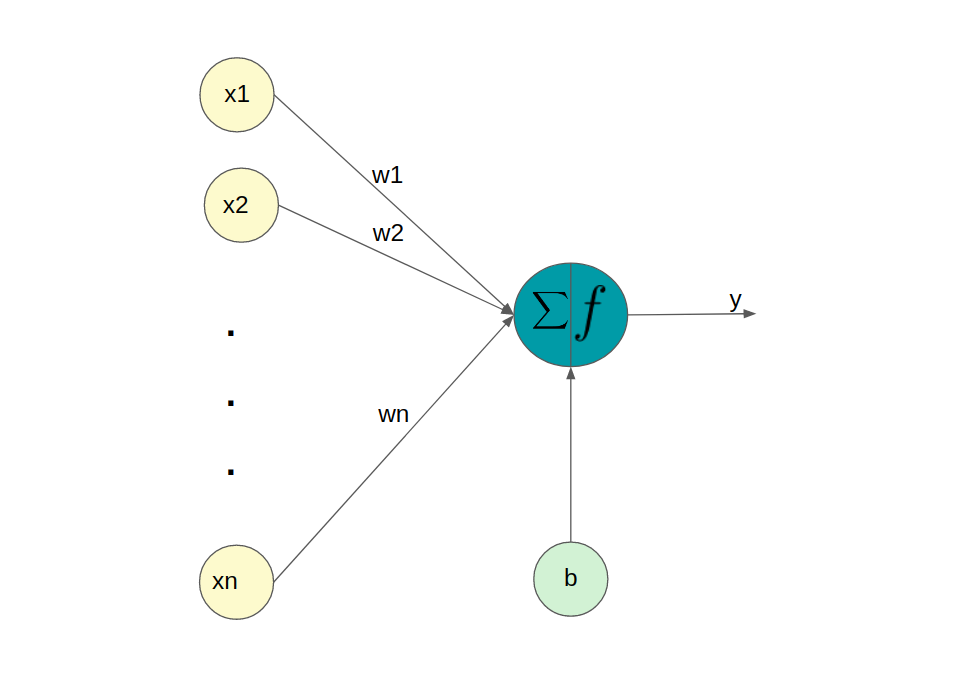
\includegraphics{figures/perceptron}
%\caption{\small \sl Perceptron.\label{fig:perceptron}} 
%\end{center} 
%\end{figure} 
%
%Jeg har implementert stochastic gradient descent i Python + PyTorch. Jeg har også laget nye implementasjoner av softmax, rectifier og kunstige neuroner i PyTorch.
%
%Fordelen med PyTorch er at den er maskinvareakselerert. Det vi si at GPU-en gjør beregningene, ikke bare CPU-en.
%
%GPU-er kommer fra dataspillindustrien. Alle datamaskiner i dag er heterogene, det vil si at de har både en CPU, en generell datahjerne, og en GPU, en grafikkdatahjerne. GPU-er er mange tusen ganger raskere enn en CPU, men kun for oppgaver som er "massively parallel". Både medisin, neurale nettverk, maskinsyn CAD, 3D animasjonsfilmproduksjon, spillutvikling og virtual reality drar nytte fra GPU-er.
%
%Det er viktig i kunstig intelligens å vite hvor et datapunkt hører hjemme. Dette gjøres med kalkulus. Mange av problemene i kunstig intelligens, og maskinsyn, er optimaliseringsproblemer. Stokastic Gradient Descent (SGD) handler om å finne en linje som passer en modell. Det er matematisk optimalisering.
%
%Jeg fikk vite om boken deeplearningboook.org , en gratis og svært god bok om deep learning. Elon Musk sier om boken: "Written by three experts in the field, Deep Learning is the only comprehensive book on the subject." (CEO SpaceX og Tesla)
%
%Jeg har lært mye om deep learning i dag. Jeg har blitt tipset om http://cs231n.stanford.edu/ og http://playground.tensorflow.org/.
%
%Som sagt så er de fleste maskinlæringsproblemer optimaliseringsproblemer. Det handler å finne ut hvor forskjellige datapunkter hører hjemme.
%
%Det finnes flere forskjellige typer problemer. Katogerisering (gi navn på data inn) og regresjon (gi et tall ut fra data inn) er typiske.
%
%Gamle neurale nettverk var perceptrons med lineære aktiveringsfunksjoner der en måtte gjøre features engineering per prosjekt for at modellen skulle virke. En kan leke med dette på tensorflow sin playground, aktiver inputs utover x1 og x2, fjern alle "hidden layers" og sett activation til linear. Test med forskjellig data. Den vil takle dataen som er i to godt avskilte skyer uten at en må tukle med features. Denne gamle måten å trene nettverkene (å finne parametere til activation featuren, for så å lage gode weights for modellen) krevde at en hadde god intuisjon om dataen en ønsket å trene nettverket på. Deep Learning med en ikke-lineær aktiveringsfunksjon gjør at den samme arkitekturen virker for alle problemer, uten feature engineering. Dette kan også lekes med, lag en eller to "hidden layers", fjern alle features untatt x1 og x2, og velg en ikke-lineær aktiveringsfunksjon. Vips, den takler alle data uten noen engineering/tweakkng, gitt nok neuroner. Tensorflow er Google sin rival til PyTorch, PyTorch er laget av Facebook.
%
%PyTorch er delvis implementert i CUDA. Dette er en GPGPU-API som fungerer kun på Nvidia GPU-er. Jeg er mer interessert i Khronos sin OpenCL-standard, som er støttet av AMD, Nvidia, Intel, samt ARM og mange mobile GPU produsenter. Jeg får bruke PC-en i stua, som har en Nvidia-GPU, når jeg trener nettverket med PyTorch.
%
%\begin{figure} 
%\begin{center} 
%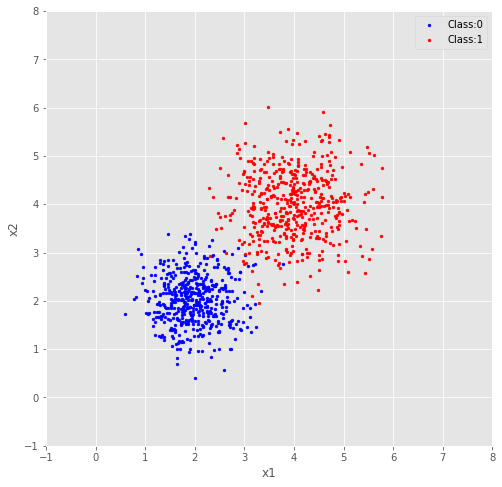
\includegraphics{figures/datapunkter}
%\caption{\small \sl Eksempel av datapunkter. De består av to forskjellige klasser, vist i rødt og blått.\label{fig:datapoints}} 
%\end{center} 
%\end{figure} 
%
%Se figur \ref{datapoints}. 
%
%\begin{figure} 
%\begin{center} 
%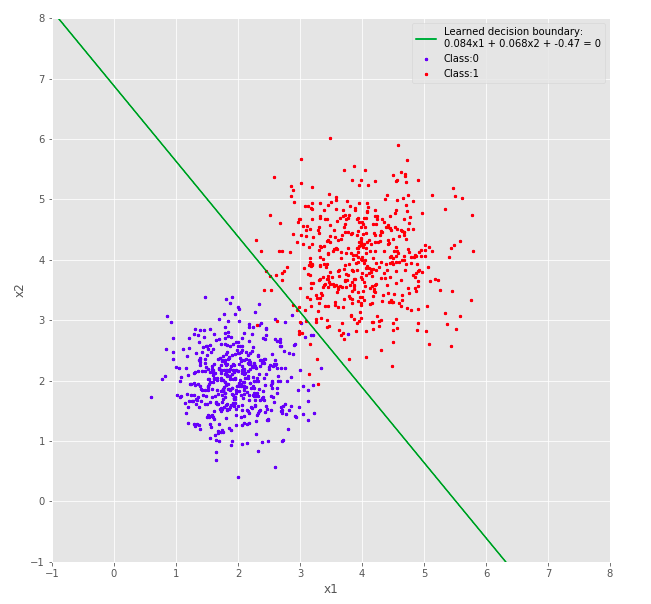
\includegraphics{figures/decision_boundary}
%\caption{\small \sl Figuren over viser decision boundary. Det er dette ML handler om, å lage denne funksjonen som skiller dataen i to grupper, her binært til gruppe 0 og 1.\label{fig:datapoints}} 
%\end{center} 
%\end{figure} 
%
%Jeg har begynt å trene opp en cnn. Jeg har en viss oversikt over deep learning nå. Det var i 2012 deep learning ble stort med AlexNet, de vant ImageNet med stor margin ved å finne på en ny måte å gjøre maskinlæring, det var deep learning.
%
%Jeg har samlet en del whitepapers som jeg skal bruke i rapporten.
%
%PyTorch har mange modeller. De har blitt veldig gode siden 2012, da måtte teamet til Geoffrey Hinton lage hele nettverket selv i CUDA. Nå er det veldig lett å lage programmer som kjenner igjen bilder med PyTorch. PyTorch gjør det også lett å laste ned test-data, og laste inn datasett, til å teste og trene modellen en velger.
%
%Det er visstnok ikke lov ("de vil se stygt på deg") å si at et kunstig neuron er som et biologisk neuron. Det er litt som å si at et fly er som en fugl. Kunstige neuroner er lignende biologiske neuroner på samme måte som fly er inspirert av fugler. 
%
%\begin{figure} 
%\begin{center} 
%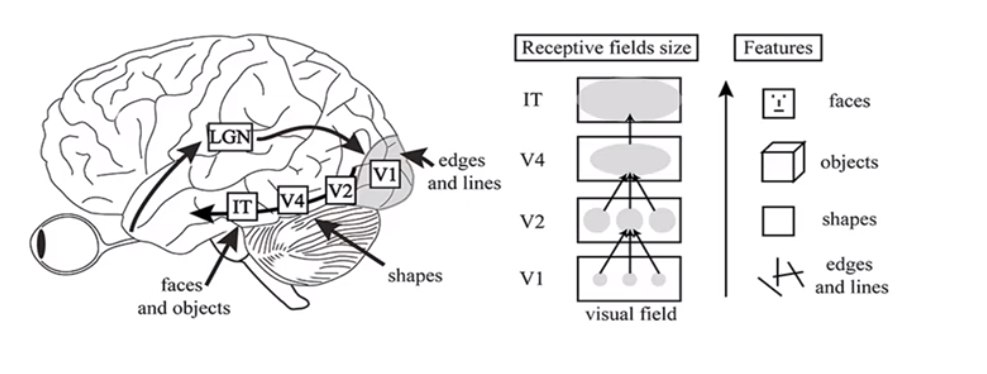
\includegraphics{figures/biological_inspiration_cnn}
%\caption{\small \sl Den biologiske inspirasjonen for cnn.\label{fig:datapoints}} 
%\end{center} 
%\end{figure} 
%
%\begin{figure} 
%\begin{center} 
%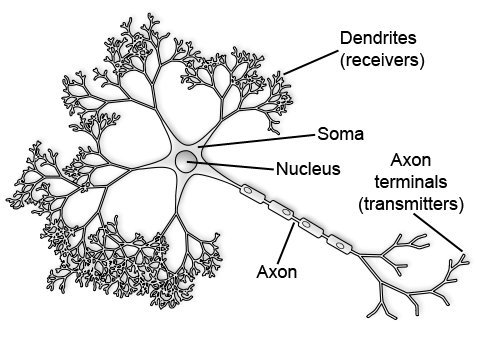
\includegraphics{figures/neuron_figure}
%\caption{\small \sl Neuron\label{fig:datapoints}}
%% https://commons.wikimedia.org/wiki/File:Neuron_figure.png
%% Nicolas.Rougier 
%\end{center} 
%\end{figure} 
%
%I dag trente jeg en ny modell og forbedret den jeg jobbet på Fredag. Denne modellen er trent med data fra PC-en min, av en panda, katt og hund. Det jeg gjorde i dag var bare en test på pipelinen og på at dataen lastes inn riktig. Jeg testet dermed kun 1 % av bildene i datasettet. Jeg fikk allikevel gode resultater. Da kan jeg gå videre.
%
%Jeg fant mange gode whitepapers på deteksjon og tracking av fisk. Å google "fish detection" gir mange resultater fra mange forskjellige prosjekter. Det blir veldig nyttig for senere.
%
%Treningen jeg skal gjøre er å lage en modell som ser forskjellen på torsk og sei. Jeg skal også lage et program som tracker og teller fisken. Å telle fisken er trivielt etter deteksjon. Dette er fine-grained detection. Jeg fant en whitepaper som tar opp spesifikt å detektere fisk av forskjellige fiskearter. Kanskje jeg låner ideer fra dem. Kan også prøve å trene deres datasett også for å få litt mer erfaring.
%
%https://www.kaggle.com/ashishsaxena2209/animal-image-datasetdog-cat-and-panda
%
%\url{https://www.researchgate.net/publication/317558591_Automatic_fish_species_classification_in_underwater_videos_Exploiting_pretrained_deep_neural_network_models_to_compensate_for_limited_labelled_data}
%
%Steg 1 - Forstå problemet
%Steg 2A - Få tak i data
%Steg 2B - Utforsk og forstå dataen
%Steg 2C - Lag et utvalg av dataen fra datasettet
%Steg 3 - Gjør klar dataen
%Steg 4 - Tren en enkel modell på datautvalget og test pipelinen før trening av et komplett nettverk påbegynnes
%Steg 5 - Tren med et komplett datasett
%Steg 6 - Iterativt forbedre modellen
%
%I dag jobbet jeg på modellen. Jeg har testet den på datasei og datatorsk. Den klarer å se forskjellen på dem med 100 \% nøyaktighet. Jeg har enda ikke gjort ferdig modellen. Jeg må fortsatt trene hele modellen, så langt så har jeg gjort steg 1-4, jeg har steg 5-6 igjen. Den neste delen av oppgaven blir å bruke modellen til objekt deteksjon og tracking i en film, slik jeg gjorde med YOLOv3 modellen tidligere.
%
%Jeg skal lage et nytt datasett med ekte torsk og sei.
%
%\begin{figure} 
%\begin{center} 
%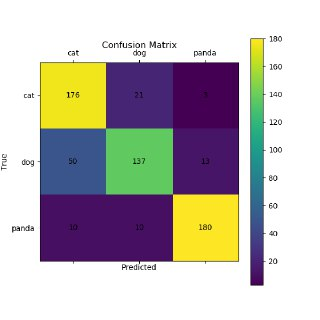
\includegraphics{figures/confusion_matrix}
%\caption{\small \sl Forvirringsmatrise. n*n. Den vil vise falske positive, sanne positive, falske negative og sanne negative for hver klasse. Om denne cnn-en var for å detektere brystkreft, og positivt sykdom betyr at en kvinne har brystkreft, så hadde falske positive vært ganske dårlig, og falske negative vært katastrofalt. En modell som, for eksempel, sier negativ hele tiden vil være 95 \% riktig, da bryskreft skjer sjeldent (i 5 \% av tilfellene, i dette tilfellet). Bias er farlig, det er viktig å balansere dataen sendt til en modell. Like mye data per klasse. \label{fig:datapoints}}
%\end{center} 
%\end{figure} 
%
%I dag implementerte jeg step-wise learning decay til modellen i et forsøk på å få bedre nøyaktighet. En modell skal ha høy learning rate i begynnelsen, så skal den bli mindre for å nå bunnen av læringskurven.
%
%Videre, å detektere fisk med maskinsyn har blitt gjort før. Det er mye bra som er skrevet om dette.
%
%Vi diskuterte hva som har gjort deep learning så populært den siste tiden. Her er nye fremskritt de siste 10 årene som har gjort deep learning populært (LeNet vs AlexNet, Andrej Karpathy 2020)
%
%\begin{figure} 
%\begin{center} 
%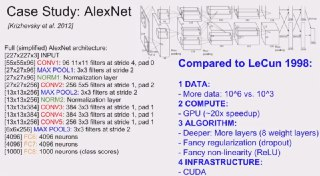
\includegraphics{figures/alexnet}
%\caption{\small \sl Vi diskuterte hva som har gjort deep learning så populært den siste tiden. Her er nye fremskritt de siste 10 årene som har gjort deep learning populært (LeNet vs AlexNet, Andrej Karpathy 2020) \label{fig:datapoints}}
%\end{center} 
%\end{figure} 
%
%Jeg har fått til YOLOv3 nå. Den går mye raskere enn RetinaNet, og kan gå i sanntid med en Nvidia GPU, slik som en 2070 gtx (regner jeg med).
%
%Jeg har brukt dagen på å se på tracking. Den må tracke flere objekter, det betyr flere trackere. En tracker krever ganske mye fra CPU-en. Det gjør programmet saktere. Men de kan multithreades. Jeg har enda ikke klart å gjøre alle fiskene som blir detektert til noe som trackes. Tracking skal være raskere enn objektdeteksjon. Jeg kan gjøre deteksjon sjeldnere enn tracking, slik at programmet går raskere. Men det må fortsatt testes. Deteksjon må uansett skje med jevne mellomrom, da nye kommer stadig inn i i bildet.
%
%Jeg har laget flere masks for segmentering, som blir et siste eksperiment, etter YOLOv3 er trent opp på sei og tracking er blitt eksperimentert med.
%
%Jeg snakket med Nofima i dag. Jeg forklarte arbeidet som jeg har gjort. Vi ble enige om å se litt mer på tracking, jeg forklarte at deteksjon uten tracking vil nok virke like bra.
%
%I dag lastet jeg opp realeases av app på github. Stein-Kato har tilgang til prosjektet nå. Jeg håper han får brukt arbeidet.
%
%Jeg har begynt å se på segmentering. Jeg håper å bli med på to kaggle konkurranser i løpet av måneden. Jeg har begynt å tenke mer på rapporten, skrivingen får nesten begynne for fullt nå, så stiller jeg bedre forberedt til BO-seminaret den 30. April.
%
%\subsubsection{Maskinlæring}
%
%Machine Learning: Learning from data
%
%Data is king.
%
%Data collection, annotation, preporation etc.
%
%Data > Algorithm > Training > Evaluation > Deployment > Predictions
%
%	Gather data from every legal source possible (public data sets, purchase data, collect data, synthesize data (super poweful))
%
%	Manually check data
%	Look for biases
%	Look for insights
%	Clean up
%
%	Iterative: Partition data 60 (training)/20 (testing accuracy training)/20 (test)
%
%Model / Algorithm
%
%	Image classification
%	Object detection 
%	Segmentation
%
%	Constraints
%
%	Experimentation (test multiple viable models)
%
%Training
%
%	Data augmentation
%	Training parameter (optimizer, rate etc.)
%	Visualizsation (check if it is going correctly)
%
%Evaluation
%	
%	Test. Check model size, speed and ACCURACY
%
%Deployment
%
%	Optimizations, deploy, feedback (know when it went badly, check failed images)	
%
%\subsubsection{Neural networks}
%
%Classification (Supervised learning)
%
%	Seperating data into groups
%
%	Binary classification (two groups) (Sigmoid activation is used)
%
%	Multiclass classification (Activation: Softmax) (Loss function: Cross entropy loss)
%
%	Regression (Activation: Linear) (Loss function: MSE loss)
%
%	Decision boundary seperates the groups by the decision function
%
%	Training is learning the decision function
%
%	Deciding decision function is called training
%
%	Data is on a plane (2D) or a hyperplane (higher dimensions)
%
%	Input layer > Hidden layer (can be many layers) > output
%
%	Each layer (node) in a nn is a neuron or perceptron
%
%	Perceptron: Calculate weighted sum of inputs and add bias. Then apply activation function (non-linear)
%
%	Every layer looks for a pattern found in the previous layer. If it is found, it "fires up"
%
%	An example of an activation function is ReLU (Rectified Linear Unit)
%
%	Another example is the sigmoid function, and tanh
%
%	An activation function creates non-linearity
%
%	The number of hidden layers is called the networks depth (depth = 2 is typical for simple problems)
%
%Loss functions
%
%	Classification outputs a category (class)
%
%	Regression outputs numerical values (or a vector of numerical values)
%
%	Many problems are optimizatino problems in ML, either to minimize or maximaze a value of a function
%
%	These functions are called the objective function
%
%	When finding the minimum, it is called a loss, or cost, function
%
%	e = y - \^y (error is ground thruth minus model output)
%
%	An error, L, can be considered either a square (MSE, most common) or an absolute number (MAE, when data has many outliers)
%
%Single layer perceptron kan løse lineære problemer
%
%Ved å gjøre "feature engineering" så kan ikke-lineære problemer løses
%
%Deep learning gjør at en kan løse lineære problemer om en bruker ikke-lineær aktivering. ReLU konvergerer raskt.
%
%%\subsubsection{Maskinsyn med OpenCV}
%%\subsubsection{Video med undervannskamera fra merdene}
%%\subsubsection{Analysere video}
%%\subsubsection{Deep Learning med OpenCV}
%%\subsubsection{PyTorch}
%%\subsubsection{Segmentere ut fisk}
%%\subsubsection{Object Detection med OpenCV}
%%\subsubsection{Object Tracking med OpenCV}
%%\subsubsection{Klassifisere hver fisk etter art}
%%\subsubsection{Registrere antall individer av hver art fortløpende}
%%\subsection{Praktisk gjennomføring}
%%\subsubsection{Programvareutvikling med maskinlæring implementert i C++}
%%\subsubsection{Videostrøm fra merdene}
%%\subsection{Resultater}
%%\subsection{Diskusjon}
%%\subsection{Konklusjon}
%%\subsection{Referanseliste}
